
\section{ Introduction}
\label{sec:06-intro}
In the previous chapter we toured loci phenomena for billiard 3-periodics. Here we continue this exploration for other for 3-periodic families in other concentric, axis-aligned ellipse pairs, shown in \cref{fig:06-six-caps}.

\begin{figure}
    \centering
    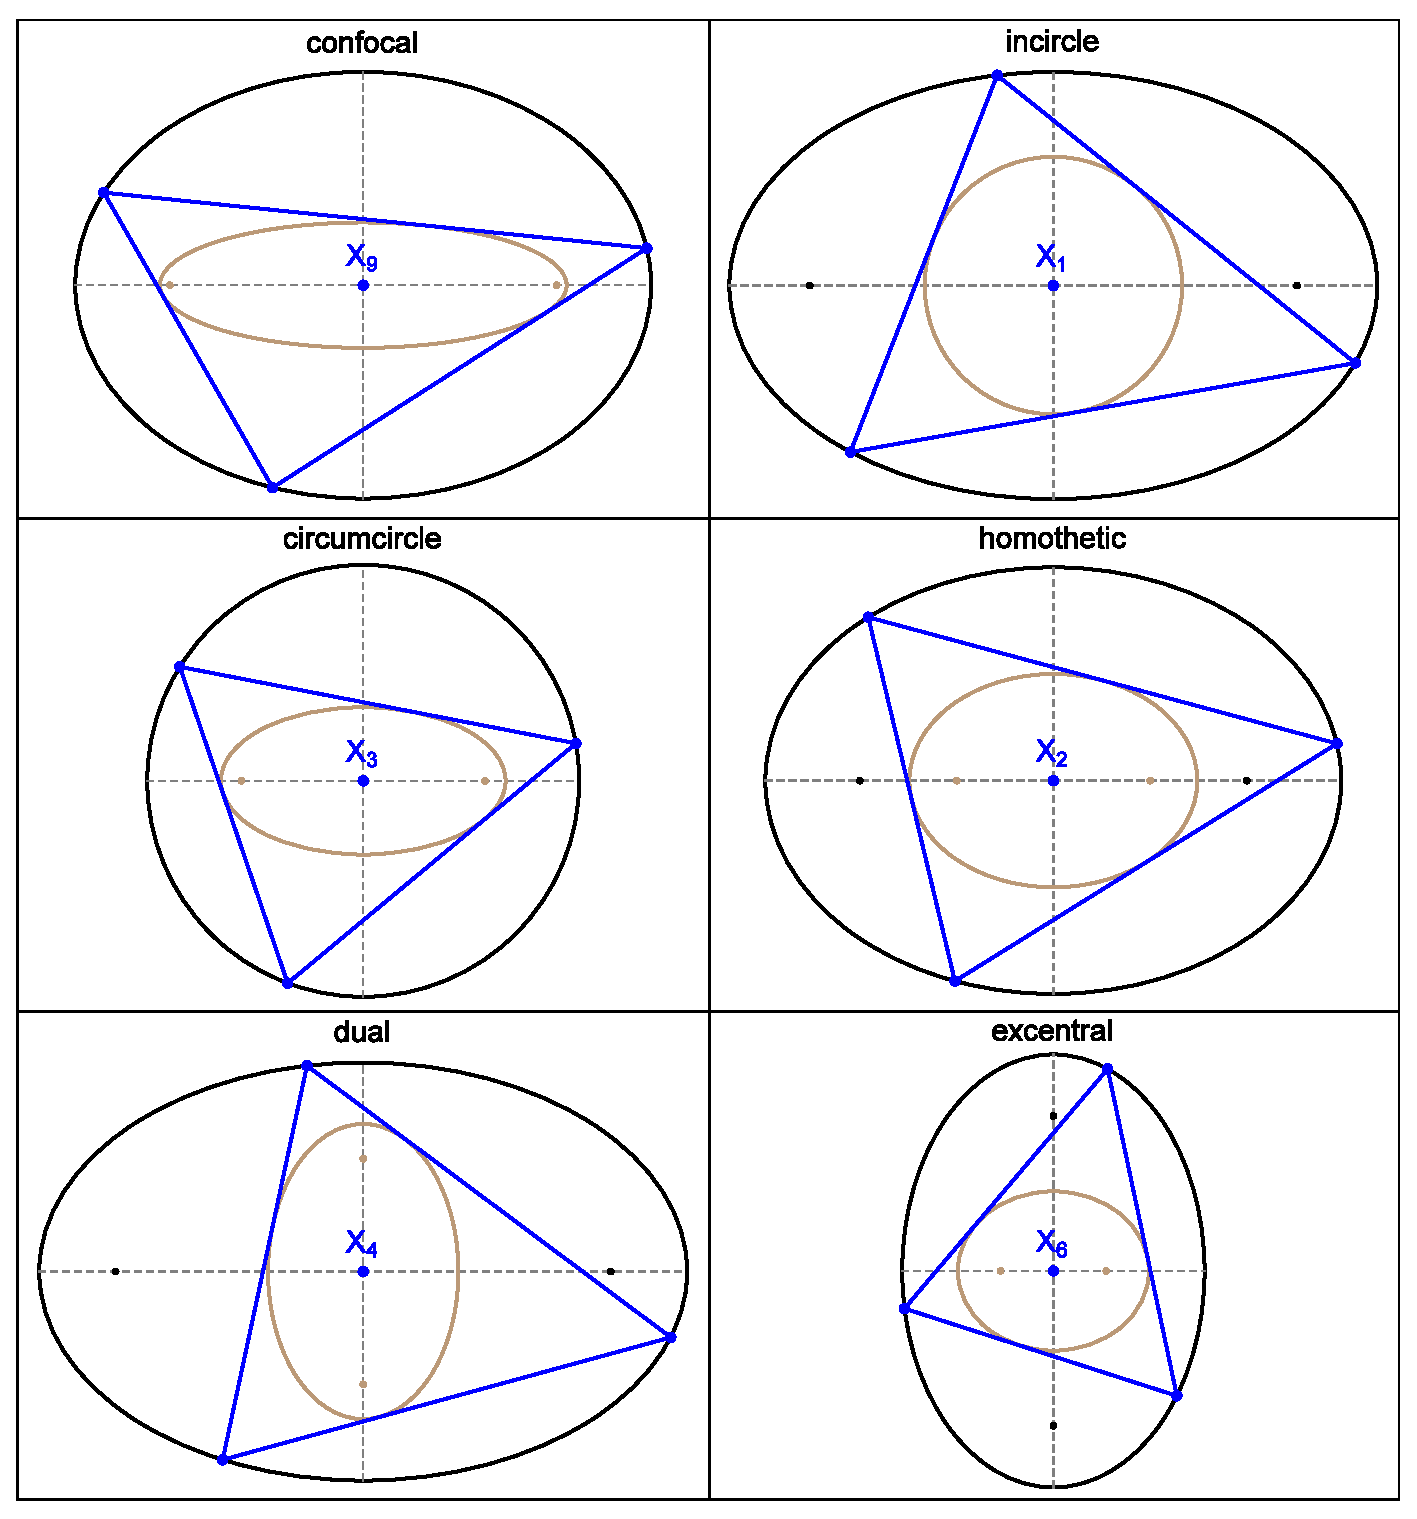
\includegraphics[width=\textwidth]{chap_06/pics/pics_06_015_six_caps_perp}
    \caption{The five concentric, axis-parallel (CAP) families whose loci are studied in this chapter. The confocal family is treated in \cref{chap:05-confocal-loci}. \href{https://youtu.be/14TQ5WlZxUw}{Video}}
    \label{fig:06-six-caps}
\end{figure}

Recall Cayley's condition for a CAP pair to admit a Poncelet 3-periodic family: $a_c/a+b_c/b=1$, where $a>b>0$, $a_c>0$, and $b_c>0$.




\section{Review: Jacobi's parametrization for bicentric polygons}
\label{sec:06-jacobi}
In 1828, Jacobi found a beautiful proof for a special case of Poncelet's closure theorem using elliptic functions. In particular, he provided a very simple parametrization for the family of N-sided bicentric polygons that appear in Poncelet's theorem. We will use his parametrization below, and it is appropriate to recall it here.

Referring to Figure~\ref{fig:jacobi-nested}, %and \ref{fig:jacobi-unnested},
consider two circles $\C_{R}$ and $\C_{r}$, with radii $R$ and $r$, respectively. Let $d$ denote the distance between their centers. We will consider polygons that are inscribed in $\C_{R}$ and also are either inscribed or exscribed in $\C_{r}$. By exscribed in $\C_{r}$ we mean that extensions of the sides of the polygon are tangent to $\C_{r}$. Let $p_{j}(u)$, $j=1,...,N$ be the vertices of a N-sided bicentric family of polygons, parametrized by the real variable $u$, with all the vertices in $\C_{R}$.

\begin{figure}
    \centering
  %  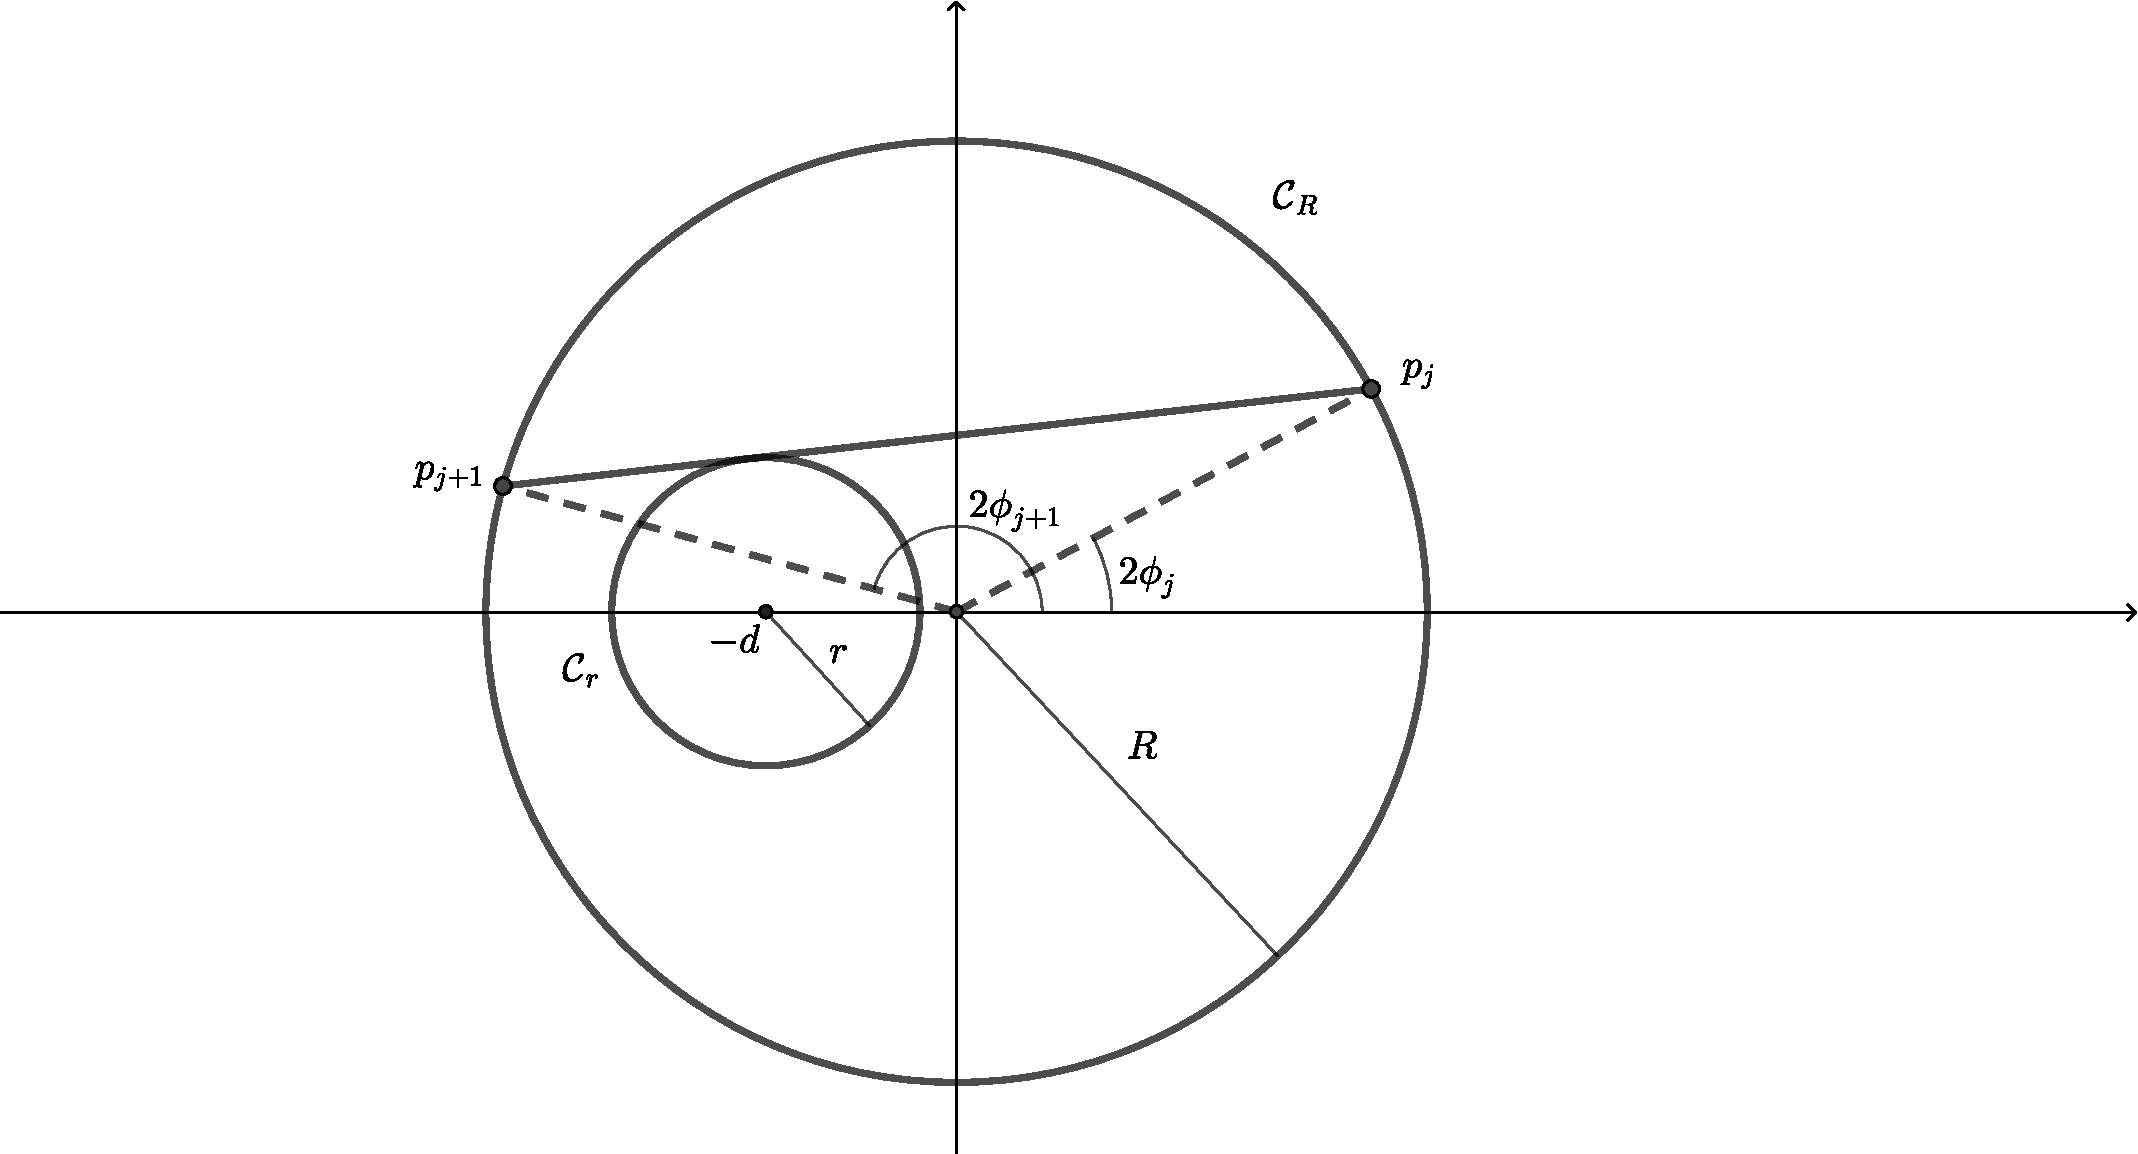
\includegraphics[width=.8\textwidth]{pics_04/0110_inscribed.pdf}
    \caption{A pair of circles, along with a chord $p_j,p_{j+1}$ of the outer circle tangent to the inner one.}
    \label{fig:jacobi-nested}
\end{figure}

%\begin{figure}
%    \centering
%    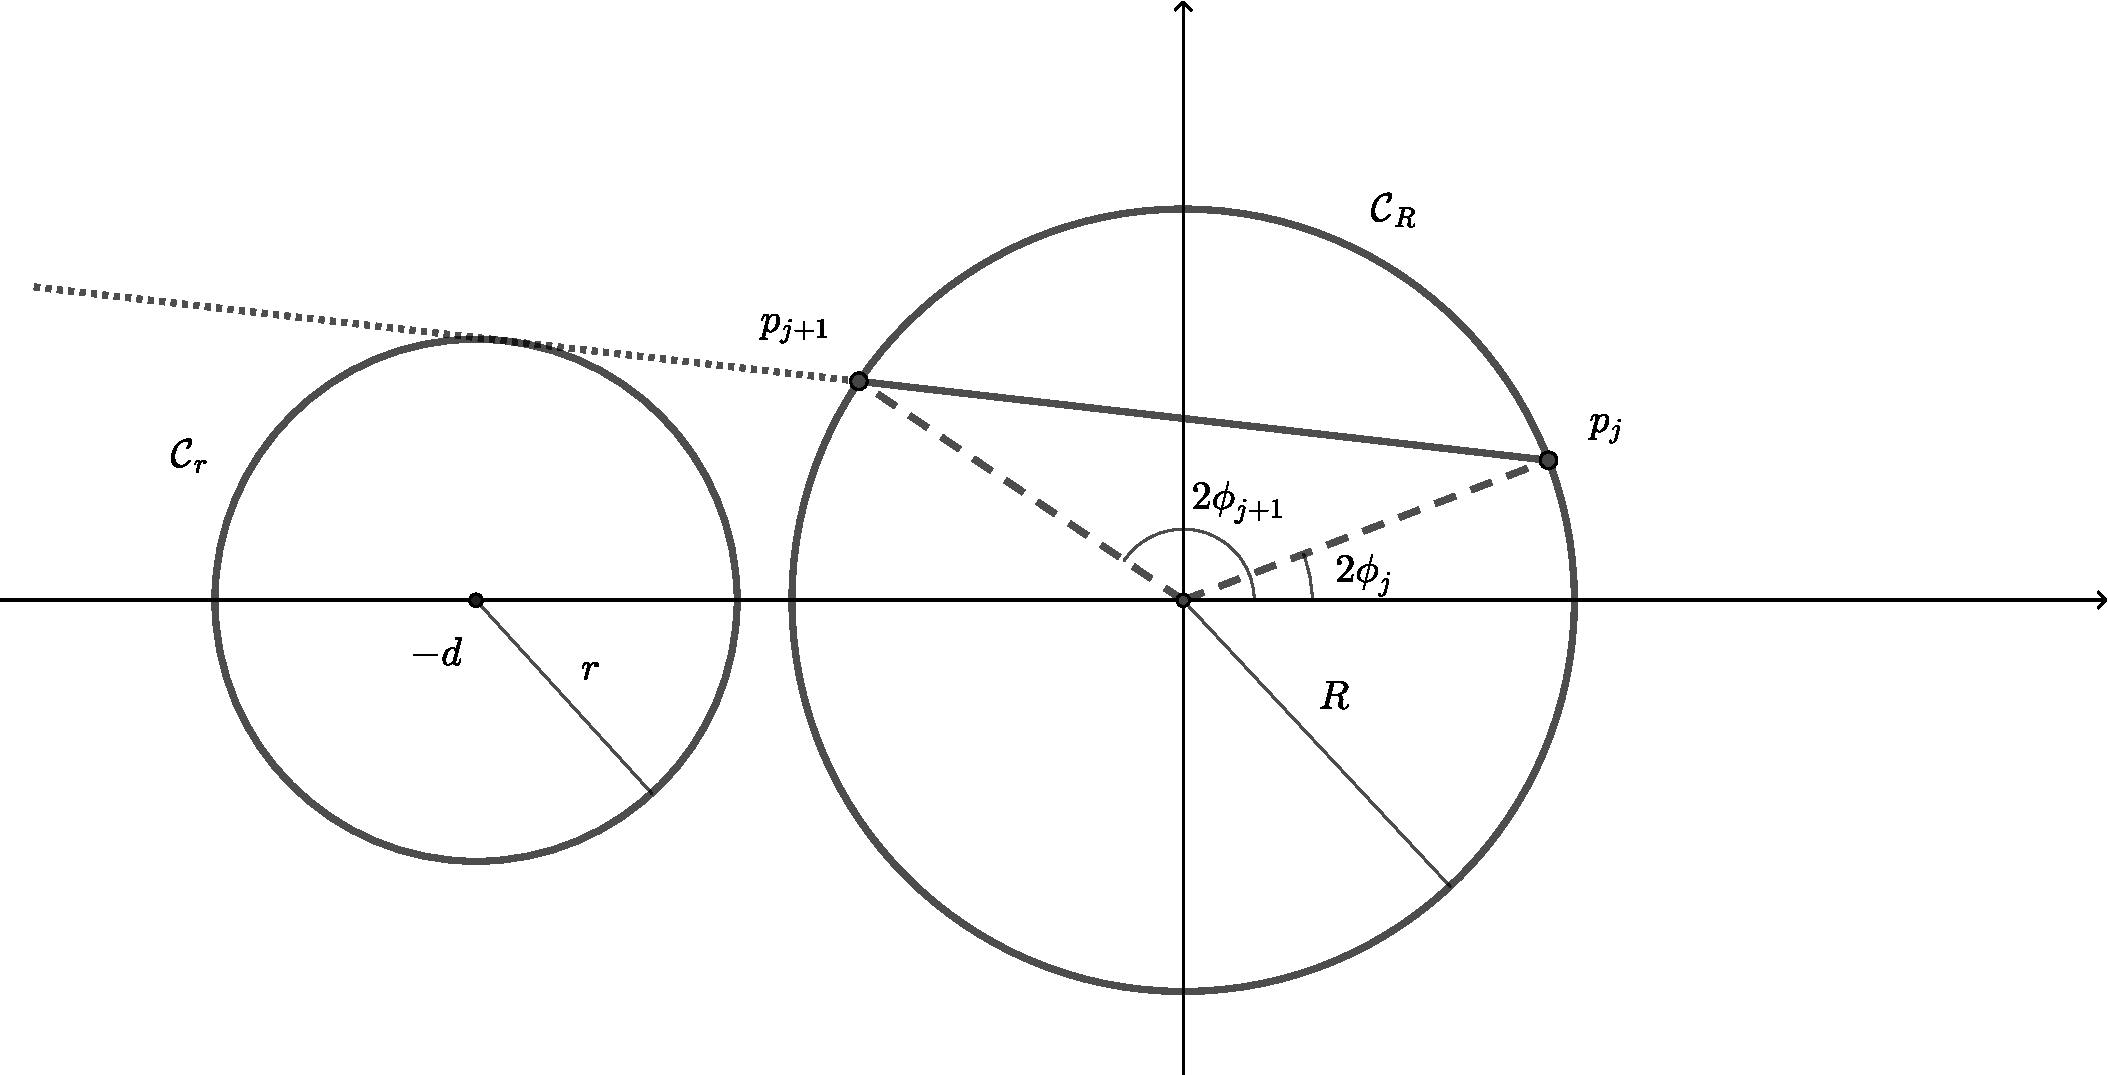
\includegraphics[width=.8\textwidth]{pics/0120_exscribed.pdf}
%    \caption{An unnested bicentric pair $\C_R$, $\C_r$.}
%    \label{fig:jacobi-unnested}
%\end{figure}

Jacobi noticed that his elliptic functions could be used to provide an explicit expression for the $p_{j}(u)$. Namely, if we write
\begin{equation}
\label{jacobivertex}  
p_{j}(u)=R\left[ \cos{(2\phi_{j}(u))}, \sin{(2\phi_{j}(u))}\right]
\end{equation}

Indeed, he proved that \cite{bos-1987}:

\begin{equation}
\label{jacobiangle}
\phi_{j}(u)=am(u+ j \sigma,k),
\end{equation}
%
where $am(u,k)$ is the classical Jacobi amplitude function \cite{armitage-2006}, $k$ is the modulus and it is related to $R$, $r$ and $d$ by the following expression \cite[pp. 315]{bos-1987}:

\begin{equation}
\label{jacobirelation}
k^2=\frac{4Rd}{(R+d)^2-r^2},\;\;\;0<k<1
\end{equation}
 %        
The real number $K$ is defined by:
%
\[K=\int_{0}^{\frac{\pi}{2}} \frac{dt}{\sqrt{1-k^2sin^2{t}}}, \]
and finally, $\sigma$ is given by

\[ \sigma=\frac{4\tau K}{N},\]
where $\tau$ is a positive integer and $N>2$.

Actually, Jacobi treated only the case where one of the circles is inscribed, but his argument also holds for the exscribed case \cite{bos-1987}.

Below we recall some very facts about three of Jacobi's elliptic functions: $sn(z,k)=\sin{(am(z,k))}$, $cn(z,k)=\cos(am(z,k))$ and $dn(z,k)=\sqrt{1-k^2sn^2(z,k)}$, where $z \in \mathbb{C}$, and $0<k<1$ is the elliptic modulus. Since $k$ is fixed, we write $sn(z)$ instead of $sn(z,k)$, etc.

These functions have two independent periods and also have simple poles at the same points. In fact:

\begin{align*}
    sn(u+4K)&=sn(u+2iK')=sn(u)\\
    cn(u+4K)&=cn(u+2K+2iK')=cn(u)\\
    dn(u+2K)&=dn(u+4iK')=dn(u)\\
    K'&=K(k'), \;\;k'=\sqrt{1-k^2}
\end{align*}
The  poles of these three functions, which are simple, occur at the points
\[2mK+i(2n+1)K'
,\;\; m,n\in \mathbb{Z}\]

They also display a certain symmetry around the poles. Namely, if $z_p$ is a pole of $sn(z)$, $cn(z)$ and $dn(z)$, then, for every $w \in \mathbb{C}$, we have \cite[Chapter 2]{armitage-2006}:

\begin{align}
sn(z_p+w)=&-sn(z_p-w) \nonumber \\
cn(z_p+w)=&-cn(z_p-w)  \label{eqn:zpole} \\
dn(z_p+w)=&-dn(z_p-w) \nonumber
\end{align}

 

\section{Bicentric Family: Invariant Sum of Cosines}
\label{sec:06-bicentric-sum-of-cosines}


\begin{theorem}
The sum of cosines of angles internal to the family of N-periodics interscribed in a bicentric pair is invariant.
\label{thm:bicentric-sum}
\end{theorem}

\begin{proof}
Let $\{p_{j}(u)\}$, as in  \eqref{jacobivertex}, denote the vertices of the family of bicentric polygons. Let $\theta_{j}(u)$ denote the internal angle at the vertex $p_{j}(u)$. It follows from elementary geometry that
$\cos{\theta_{j}(u)}=-\cos({\phi_{j+1}(u)-\phi_{j-1}(u)}).$
Thus, if we denote by $S(u)$ the sum of the cosines of the internal angles, we have:

\begin{equation}
\label{sumofcosines}
S(u)=\sum \cos{\theta_{j}(u)}=-\sum{cn(u_{j+1})cn(u_{j-1})+sn(u_{j+1})cn(u_{j-1})},
\end{equation}
where $u_{j}=u+j\sigma$.

We now consider the natural complexified version of $S(u)$ defined on the complex plane by assuming that $u$ is a complex variable. To prove that $S$ is constant, it is sufficient to show that it has no poles and then apply Liouville's theorem.

So, suppose that $u=u_p$ is a pole of $S$. This implies that, for a certain index $j$, $u_{j}=u_{p}+j\sigma$ is a common pole of $cn(z)$ and $sn(z)$. We will now see that this leads to a contradiction.

In fact, by looking at (\ref{sumofcosines}), the terms where $u_{j}$ appears are given by
$$-(cn(u_{j})cn(u_{j-2})-sn(u_{j})cn(u_{j-2})+cn(u_{j+2})cn(u_{j})-sn(u_{j+2})cn(u_{j})).$$

Thus, the coefficients of $cn(u_{j})$ and $sn(u_{j})$ are, respectively:

$$-(cn(u_{j-2})+cn(u_{j+2})),$$

$$-(sn(u_{j-2})+sn(u_{j+2})).$$

Note that by (\ref{eqn:zpole}) both coefficients are zero, and they cancel out the simple poles of $cn(z)$ and $sn(z)$ at $u_{j}$, so $u_{p}$ is not a pole of $S$.   
\end{proof}

  

 %\section{Bicentric Limiting Pedals: Invariant Perimeter}
%\label{sec:pedal-perimeter}
%\section{Main Result}

History of experiment. Pedro found out about our work via Youtube (insomnia). Asked us about an invariant involving billiard curvatures at the vertices, we found $\sum{k^{2/3}}$ but this is a direct corollary of the sum of cosines. This implied $\sum{1/(d_1 d_2)}$ was invariant. Jair gave the idea to check if the stronger result $\sum{1/d_1}$ was invariant, which it was. This corresponds to the sum of the inverse lengths of ``focal spokes'', or the sum of the lengths of the focal spokes to the inversive polygon, both which are invariant. We then simply tested the perimeter of the inversive polygon which was unexpectedly constant.

In \cite{reznik2020-n3-focus-inversive} we showed:

\begin{theorem}
Over 3-periodics in the elliptic billiard (confocal pair) the perimeter of the focus-inversive polygon is invariant and given by:

\[ ... \]

Furthermore the inversive family is a 3-periodic of a rigidly rotating elliptic billiard whose axes are given by:

\[ ... \]


\end{theorem}

\begin{theorem}
Over N-periodics in the elliptic billiard (confocal pair) the perimeter of the focus-inversive polygon is invariant.
\end{theorem}

\section{Proof by Jacobi Elliptic Functions}


\begin{lemma}
The polar curve of the ellipse $\mathcal{E}$ is the circle
\begin{align*}
   C(x,y)&= (x +\frac{c(b^2 + \rho^2)}{b^2})^2+y^2-\frac{a^2\rho^4}{b^4}=0\\
  % x_0&=  -\frac{c(b^2 + r^2)}{b^2}
    %  x_0&=-\frac{(a - b)(ab + b^2 + r^2)}{bc}\\
\end{align*}  
\end{lemma}

\textcolor{red}{ron:checar x0 abaixo}
\begin{lemma}
The polar curve of the hyperbola $\mathcal{H}$ is the circle
\begin{align*}
   C(x,y)&= \left(x- \frac{c(\rho^2 - b^2)}{b^2} \right)^2+y^2-\frac{a^2\rho^4}{b^4}=0\\
 %  x_0&=  \frac{c(r^2 - b^2)}{b^2} 
\end{align*}  
\end{lemma}

\begin{lemma}
The limit points of a pair of polar circles associated to a pair of confocal ellipes are
\[ \left[-c,0\right], \;\; \left[-c+\frac{\rho^2}{c} ,0\right]\]

\end{lemma}
\section{Mapping a Confocal to a Bicentric Pair}
Under the polar transformation an origin-centered ellipse $\E$ is sent to the circle:

\[ \left( x+{\frac {c \left( {b}^{2}+\rho^{2} \right) }{{b}^{2}}}
 \right) ^{2}+{y}^{2}-{\frac {{a}^{2}\rho^{4}}{{b}^4}}=0\]
 and the confocal ellipse $\E_c$ is sent to
 \[ \left( x+\frac {c \left( b_c^{2}+\rho^{2} \right) }{b_c^2}
 \right) ^{2}+{y}^{2}-{\frac {a_c^{2}\rho^{4}}{b_c^4}}=0\]
 
Therefore:

\begin{align*} r&=\frac{a \,\rho^2}{b^2},\; R=\frac{a_c\, \rho^2}{b_c^2}\\
d&=\frac {c \left( b_c^{2}+\rho^{2} \right) }{b_c^2}-\frac {c \left( b^{2}+\rho^{2} \right) }{b^2}=\frac{c \rho^2(b^2 - b_c^2)}{b^2\, b_c^2}=\frac{\rho^2 c\, (a^2 - a_c^2)}{b^2\, b_c^2}\\
  k^2&=\frac{4Rd}{(R+d)^2-r^2}=\frac{4 \,c\, a_c\,(a_c - c)^2    }{b_c^4}\\
  \delta_{\pm}&=\pm {\frac {\rho^{6}{a}^{4}}{2\,c\, {b}^{8}}}+{\frac { \left( {a}^{2} b_c^{4}-a_c^{2}{b}^{4}-{c}^{6} \right) \rho^{2}}{2\,{b}^{2}  b_c^{2} {c}^{3}}}
\end{align*}

 The limiting points $\ell_1,\ell_2$ are given by: $[-c,0]$ and $[-c+\frac{\rho^2}{c},0]$.
 
 
 \textcolor{red}{Ron: calculos abaixos foram simplificados na secao seguinte}
 
 
 Reciprocally, given a pair of circles $C_R:\; (x+d)^2+y^2=R^2$ and $C_r:\; x^2+y^2=r^2$, by the  polar transformation, 
 it is associated a pair of confocal ellipses $\{\E, \E_c\}$
 with semiaxes given by:
 
 \begin{align*}
     a&= \sqrt{b^2+c^2}=\frac{\sqrt{2}\rho^2\sqrt{ (R^2 - d^2 - r^2)\sqrt{\alpha} +(R^2 - d^2)^2  - r^2(2R^2 - r^2) }}{2r\alpha} \\
     b&= {\frac {\sqrt {2}{\rho}^{2}}{2\,\alpha\,r}\sqrt {\alpha\, \left( 
\alpha+\sqrt {4\,\alpha\,{r}^{2}{d}^{2}+{\alpha}^{2}} \right) }}
 \\
     a_c&= \sqrt{b_c^2+c^2} = \frac{\sqrt{2}\rho^2\sqrt{(R^2 + d^2 - r^2)\sqrt{\alpha} + R^2(R^2 - 2r^2) + (d^2 - r^2)^2 }}{2R\alpha}\\
     b_c&= {\frac {\sqrt {2}{\rho}^{2}}{2 \alpha\,R}\sqrt {\alpha\, \left( \alpha+
\sqrt {4\,\alpha {R}^{2}\,{d}^{2}+{\alpha}^{2}} \right) }}
 \\
     c&= {\frac {d{\rho}^{2}}{2\,\alpha\, \left( R^2-r^2 \right)    } \left( \sqrt {\alpha\, \left( 4\, {r}^{2} d^2+\alpha
 \right) }+\sqrt {\alpha\, \left( 4\,{R}^{2}{d}^{2}+\alpha \right) }
 \right) }
\\
     \alpha&=(R - d + r)(R + d + r)(R - d - r)(R + d - r)
 \end{align*}
 
 Under the polar transformation an origin-centered ellipse $\E$ is sent to the circle:

\[ \left( x+{\frac {c \left( {b}^{2}+\rho^{2} \right) }{{b}^{2}}}
 \right) ^{2}+{y}^{2}-{\frac {{a}^{2}\rho^{4}}{{b}^4}}=0\]
 and the confocal ellipse $\E_c$ is sent to
 \[ \left( x+\frac {c \left( b_c^{2}+\rho^{2} \right) }{b_c^2}
 \right) ^{2}+{y}^{2}-{\frac {a_c^{2}\rho^{4}}{b_c^4}}=0\]
 
Therefore:

\begin{align*} r&=\frac{a \,\rho^2}{b^2},\; R=\frac{a_c\, \rho^2}{b_c^2}\\
d&=\frac {c \left( b_c^{2}+\rho^{2} \right) }{b_c^2}-\frac {c \left( b^{2}+\rho^{2} \right) }{b^2}=\frac{c \rho^2(b^2 - b_c^2)}{b^2\, b_c^2}=\frac{\rho^2 c\, (a^2 - a_c^2)}{b^2\, b_c^2}\\
  k^2&=\frac{4Rd}{(R+d)^2-r^2}=\frac{4 \,c\, a_c\,(a_c - c)^2    }{b_c^4}\\
  \delta_{\pm}&=\pm {\frac {\rho^{6}{a}^{4}}{2\,c\, {b}^{8}}}+{\frac { \left( {a}^{2} b_c^{4}-a_c^{2}{b}^{4}-{c}^{6} \right) \rho^{2}}{2\,{b}^{2}  b_c^{2} {c}^{3}}}
\end{align*}

 The limiting points $\ell_1,\ell_2$ are given by: $[-c,0]$ and $[-c+\frac{\rho^2}{c},0]$.
 
 
 \section{ Hyperbolas}
 
 Consider the pair of circles $x^2+y^2=r^2$
 and $(x+d)^2+y^2=R^2$ and the limit points
 $\ell_1= (R^2 - d^2 - r^2 -\Delta)/(2d)$ and $\ell_2=(R^2 - d^2 - r^2 + \Delta)/(2 d)$,
where
 \[ \Delta=\sqrt { \left( d+R+r \right)  \left( R-d+r \right)  \left( R+d-r
 \right)  \left( R-d-r \right) }\]

 \begin{lemma} The polar image of the circle $x^2+y^2=r^2$ with respect to the limit point $  \ell_2 $ is the hyperbola  centered at
 \[ \left[\frac{\Delta^2-2d^2k^2  }{2 d \Delta} + \frac{R^2 - d^2 - r^2}{ 2 d },0\right] \]
 and semiaxes given by
 
 \begin{align*}
     a^2&=\frac{k^4(   2d^2r^2-\Delta(R^2 - d^2 - r^2 - \Delta))}{2 r^2 \Delta^2}\\
     b^2&= \frac{k^4(R^2 - d^2 - r^2 - \Delta)}{2 \Delta r^2  } \\
     c^2&=a^2+b^2=\frac{k^4d^2}{\Delta^2}
 \end{align*}
 \end{lemma}
 
 
 \begin{lemma} The polar image of the circle $(x+d)^2+y^2=R^2$ with respect to the limit point $  \ell_2 $ is the hyperbola  centered at
 \[ \left[\frac{\Delta^2-2d^2k^2  }{2 d \Delta} + \frac{R^2 - d^2 - r^2}{ 2 d },0\right] \]
 and semiaxes given by
 
 \begin{align*}
     a^2&= \frac{k^4(2R^2d^2 - \Delta (R^2 + d^2 - r^2 - \Delta))}{ 2R^2 \Delta^2} \\
     b^2&=  \frac{(R^2+  d^2 - r^2 - \Delta)k^4}{ 2 \Delta R^2} \\
     c^2&=a^2+b^2=\frac{k^4d^2}{\Delta^2}
 \end{align*}
 \end{lemma}


\begin{lemma} The polar image of the circle $x^2+y^2=r^2$ with respect to the limit point $  \ell_1 $ is the ellipse  centered at
 \[ \left[ \frac{ 2 d^2 k^2 - \Delta^2}{ 2 \Delta d} + \frac{R^2 - d^2 - r^2}{ 2 d},0\right] \]
 and semiaxes given by
 
 \begin{align*}
     a^2&=\frac{( (\Delta + R^2 - d^2 - r^2)\Delta + 2d^2r^2)k^4}{ 2 \Delta r^2} \\
     b^2&=\frac{    (R^2+ \Delta-d^2 - r^2 ) k^4}{2 \Delta r^2} \\
     c^2&=a^2-b^2=\frac{k^4d^2}{\Delta^2}
 \end{align*}
 \end{lemma}
 
 
 \begin{lemma} The polar image of the circle $(x+d)^2+y^2=R^2$ with respect to the limit point $  \ell_1 $ is the ellipse centered at
 \[ \left[ \frac{ 2 d^2 k^2 - \Delta^2}{ 2 \Delta d} + \frac{R^2 - d^2 - r^2}{ 2 d},0\right] \]
 and semiaxes given by
 
 \begin{align*}
     a^2&= \frac{(2R^2d^2 + \Delta (  \Delta+R^2 + d^2 - r^2 ))k^4}{ 2 \Delta R^2}  \\
     b^2&=  \frac{(\Delta+R^2 + d^2 - r^2   )k^4}{ 2 \Delta R^2} \\
     c^2&=a^2-b^2=\frac{k^4d^2}{\Delta^2}
 \end{align*}
 \end{lemma}

 
\section{Poristic}

\begin{definition}
Let $\P=\{p_1,\ldots p_n\}$ be an $n-$gon with vertices  $p_i$ with $p_{n+1}=p_1$. From each vertex $p_i$ draw a perpendicular to the segment $p_{i-1}p_{i+1}$ .
In general, these perpendiculars have no
common point, but when  they meet at a single point,   this point will be   called
the orthocentre of the $n-$gon  $\P$.
\end{definition}
\begin{theorem}
Let $\Gamma$   be the circle inscribed in an n-gon $\P$, let $I$ be the inversion with
respect to $\Gamma$, $a_i$ the centres of the circles equal to the $I-$images of the straight lines
containing sides of $\P$ , and let $A$ be the base $n-$gon with vertices $a_i$. The polygon $\P$
admits a circumscribed circle $\C$ if and only if the corresponding base $n-$gon $A$ has
an orthocentre. This orthocentre is the centre of the circle
$I(\C)$, the image of the
circumscribed circle $\C$ under $I$ .
\end{theorem}

Pedro's paper.

\section{Future Work}

\begin{conjecture}
Over N-periodics in the elliptic billiard, the sum of cosines of the inversive polygon is invariant except for simple $N=4$.
\end{conjecture}

\begin{conjecture}
The product of areas of the two focus-inversive polygons is invariant for all odd $N$. 
\end{conjecture}

\begin{conjecture}
The ratio of areas of polar to inversive polygons is invariant for all $N$. 
\end{conjecture}
  

\section{Bicentric Limiting Pedals: Invariant Perimeter}
\label{sec:06-pedal-perimeter}
In this section we prove that the two pedal polygons of a bicentric Poncelet family with respect to circles centered on either of its two {\em limiting points} (see below) conserve perimeter.

\begin{definition}[Pedal Polygon]
Given a planar polygon $\P$ and a point $p$, the {\em pedal polygon} $\P_{\perp}$ of $\P$ wrt $p$ has vertices $q_{j}$ at the orthogonal projections of $p$ onto the jth sideline $p_{j}p_{j+1}$ or extension thereof.
\end{definition}

\begin{definition}[Limiting Point]
Any pair of circles is associated with a pair of ``limiting'' points $\ell_1,\ell_2$ which lie on the line connecting the centers, with respect to which the circles are inverted to a concentric pair.
\end{definition}

Let $\C_{R}$ be a circle of radius $R$ centered at the origin $(0,0)$ and $\C_{r}$ be a circle of radius $r$ centered at $(-d,0)$. Then the limiting points $(\delta_{\pm},0)$ of the pencil of circles defined by $\C_{R}$ and $\C_{r}$ has abscissa given by \cite[Limiting Point, Eqn. 5]{mw}:

\begin{equation}
\delta_{\pm}=\frac{r^2-R^2-d^2 \pm %\sqrt{R^4-2R^2d^2-2R^2r^2+d^4-2d^2r^2+r^4}}{2d}
\sqrt{d^4 -2(R^2 +r^2)d^2 + (R^2 - r^2)^2 }}{2d}
\label{eqn:limiting-point}
\end{equation}

Let $\P(u)$ be the family of bicentric polygons with respect to a pair of circles $C_{R}$ and $C_{r}$, where $u$ is the real parameter introduced by Jacobi, with vertices given by (\ref{jacobivertex}). Let $\ell$ denote a limiting point of the pencil defined by these circles, as in \eqref{eqn:limiting-point}. Below we derive an expression for the length of the sides of pedal polygons  $\P_{\perp}(u)$ defined by $\P(u)$ and $\ell$.

\begin{lemma}
\label{lem:pedal-perimeter}
 Let $p_{j-1}(u)$, $p_{j}(u)$ and $p_{j+1}(u)$ be three consecutive vertices of $\P(u)$, let $s_{j}(u)=|q_{j+1}(u)- q_{j}(u)|$ be jth sidelength of $\P_{\perp}$. Then:

\begin{equation}
\label{pedalside}
s_{j}(u)=\frac{r_{j}(u)\rho_{j}(u)}{2R},
\end{equation}
%
where $r_{j}(u)=\left|p_{j-1}(u)-p_{j+1}(u)\right|$ and $\rho_{j}(u)=\left|\ell-p_{j}(u)\right|$. In addition, $r_{j}(u)$ and $\rho_{j}(u)$ are given by the following expressions.
  
\begin{align}
r_{j}(u)=&2R\sin{(\phi_{j+1}(u)-\phi_{j-1}(u))} \label{sideterm} \\
=&2R\left(sn(u_{j+1})cn(u_{j-1})-sn(u_{j-1})cn(u_{j+1})\right) \nonumber
\end{align} 
where $u_{j}=u+j \sigma$.

\begin{equation}
\label{spoketerm}
\rho_{j}(u)=\frac{2}{k}\sqrt{-\delta_{\pm}R}\,\,dn(u_{j}).
\end{equation}
\end{lemma}
\begin{proof}
The proof of \eqref{pedalside} follows the standard one for sidelengths of the pedal triangle \cite[pp. 135--141]{johnson1960}. Equation \eqref{sideterm} follows by inspection from \cref{fig:jacobi-nested}, and the definition of Jacobi's $sn(u)$ and $cn(u)$. Finally, \eqref{spoketerm} is a long but simple computation. Below we show a few intermediate steps. First, if we let $\ell=(\delta_{\pm},0)$ be either limiting point. Then:

\[\rho_{j}(u)=\cos(\phi_{j}(u))\sqrt{R^2-2R\delta_{\pm}}+\delta_{\pm}^2\]

It is straightforward to check that $\delta_{\pm}<0$. Substitute the expression \eqref{eqn:limiting-point} for $\delta_{\pm}$ in the expression for $\rho_{j}(u)$ to obtain:

\[\rho_{j}(u)=\sqrt{\frac{-\delta_{\pm}}{d}\Big( R^2+d^2-r^2-2Rd\cos{(2\phi_{j}(u))}\Big)}\]

Finally, using \eqref{jacobirelation}, we get:

\[\rho_{j}(u)=\frac{2}{k}\sqrt{-\delta_{\pm}R}\sqrt{1-k^2sn^2(u_{j})}=\frac{2}{k}\sqrt{-\delta_{\pm}R}\,\,dn(u_{j})\] 
\end{proof}

We are now in a position to prove the following.

\begin{theorem}
The perimeters $L_\pm$ of the pedal polygons of the bicentric Poncelet family with respect to either limiting point are invariant.
\label{thm:bicentric-pedal-perimeter}
\end{theorem}

\begin{proof}
From Lemma \ref{lem:pedal-perimeter}, the perimeter is given by:

\[ L_\pm(u)=\frac{\sqrt{-\delta_{\pm}R}}{k}\sum{dn(u_{j})\Big(sn(u_{j+1})cn(u_{j-1})-sn(u_{j-1})cn(u_{j+1})\Big)} \]

To prove the above is constant, we consider its natural complexified version, that is, we think of $L_\pm$ as function of a complex variable $u$. Clearly, $L_\pm$ becomes a meromorphic function defined on the complex plane. To prove that $L_\pm$ is constant we will show that it is entire and bounded. So by Liouville's theorem it must be constant.

In turn this amounts to showing $L_\pm$ has no poles. Now, suppose that, for $u=u_p$, a certain $u_{j}$ is a common simple pole of $sn(z)$, $cn(z)$ and $dn(z)$. This is the only way that $L_\pm$ can have a pole.

From the expression of $L_\pm$, it follows there are three terms in the sum where the pole $u_{j}$ of the three Jacobian elliptic functions appears:

\begin{align*}
dn(u_{j-1})&\left(sn(u_{j})cn(u_{j-2})-sn(u_{j-2})cn(u_{j})\right)\\
dn(u_{j})&\left(sn(u_{j+1})cn(u_{j-1})-sn(u_{j-1})cn(u_{j+1})\right)\\
dn(u_{j+1})&\left(sn(u_{j+2})cn(u_{j})-sn(u_{j})cn(u_{j+2})\right)
\end{align*}

We have to prove that the sum of these terms is finite at $u_{j}$. To see this, consider first the term that multiplies $dn(u_{j})$, namely

\[sn(u_{j+1})cn(u_{j-1})-sn(u_{j-1})cn(u_{j+1}).\]

Since $u_j=u+j \sigma$ is a pole and   $u_{j+1}=u_j+ \sigma$, $u_{j-1}=u_j- \sigma$ it follows from \eqref{eqn:zpole} that  $sn(u_{j-1})=-sn(u_{j+1})$ and $cn(u_{j-1})=-cn(u_{j+1})$. Therefore, the expression above is zero. And this cancels the simple pole of $dn(u)$ at $u_{j}$. The same argument can be applied to the terms that multiply $sn(u_{j})$ and $cn(u_{j})$ and this shows that $u_p$ is not a pole of $L_\pm$. 

So $L_\pm$ has no poles and by the periodicity of the elliptic functions, it must be bounded. Thus, by Liouville's theorem $L_\pm$ is constant.
\end{proof}

%In Appendix~\ref{app:explicit-perimeter} we provide explicit %expressions (in terms of Jacobi elliptic functions) for $L_\pm$.

In \cref{app:bicentric-to-confocal,app:confocal-to-bicentric} we show that the image of two nested circles wrt to $\ell_1$ is a confocal pair of ellipses, therefore under this tranformation, a bicentric N-gon is sent to an elliptic billiard N-gon. Lemmas \ref{lem:polar} and \ref{lem:limit-focus} found in the Appendix~\ref{app:polar-pedal} show that the bicentric pedal with respect to $\ell_1$ is identical to its polar image (elliptic billiard N-periodic) inverted with respect to a circle centered on $f_1=\ell_1$. Therefore:

\begin{corollary}
Over the family of N-periodics in the elliptic billiard (confocal pair), the perimeter of inversions of said N-periodics with respect to a focus-centered circle is invariant. 
\label{cor:inv-per}
\end{corollary}


Though not yet proved, experimental evidence suggests:

\begin{conjecture}
The sum of cosines of bicentric pedal polygons with respect to either limiting point is invariant, except for the $\ell_1$-pedal in the $N=4$ case.
\label{conj:limiting-sum-cosines}
\end{conjecture}  

\section{A Tale of Five Polygons}
\label{sec:06-five-polys}
Illustrated in \cref{fig:five-polys} is the bicentric family along with its two limiting-pedals and its two polar images (elliptic and hyperbolic billiards), each with respect to a limiting point. While N-periodics in the elliptic billiard conserves perimeter, it turns out their hyperbolic versions conserve their {\em signed} perimeter, i.e., the length of segments on where both (just one) coordinates change sign are counted as negative (resp. positive).

Indeed \cref{fig:bicentric-diagram} illustrates that the bicentric family is a kind of ``hub'' from which four equiperimeter (and of constant cosine sum) derived polygon families can be obtained. Bicentrics themselves have variable perimeter.

\begin{figure}
    \centering
    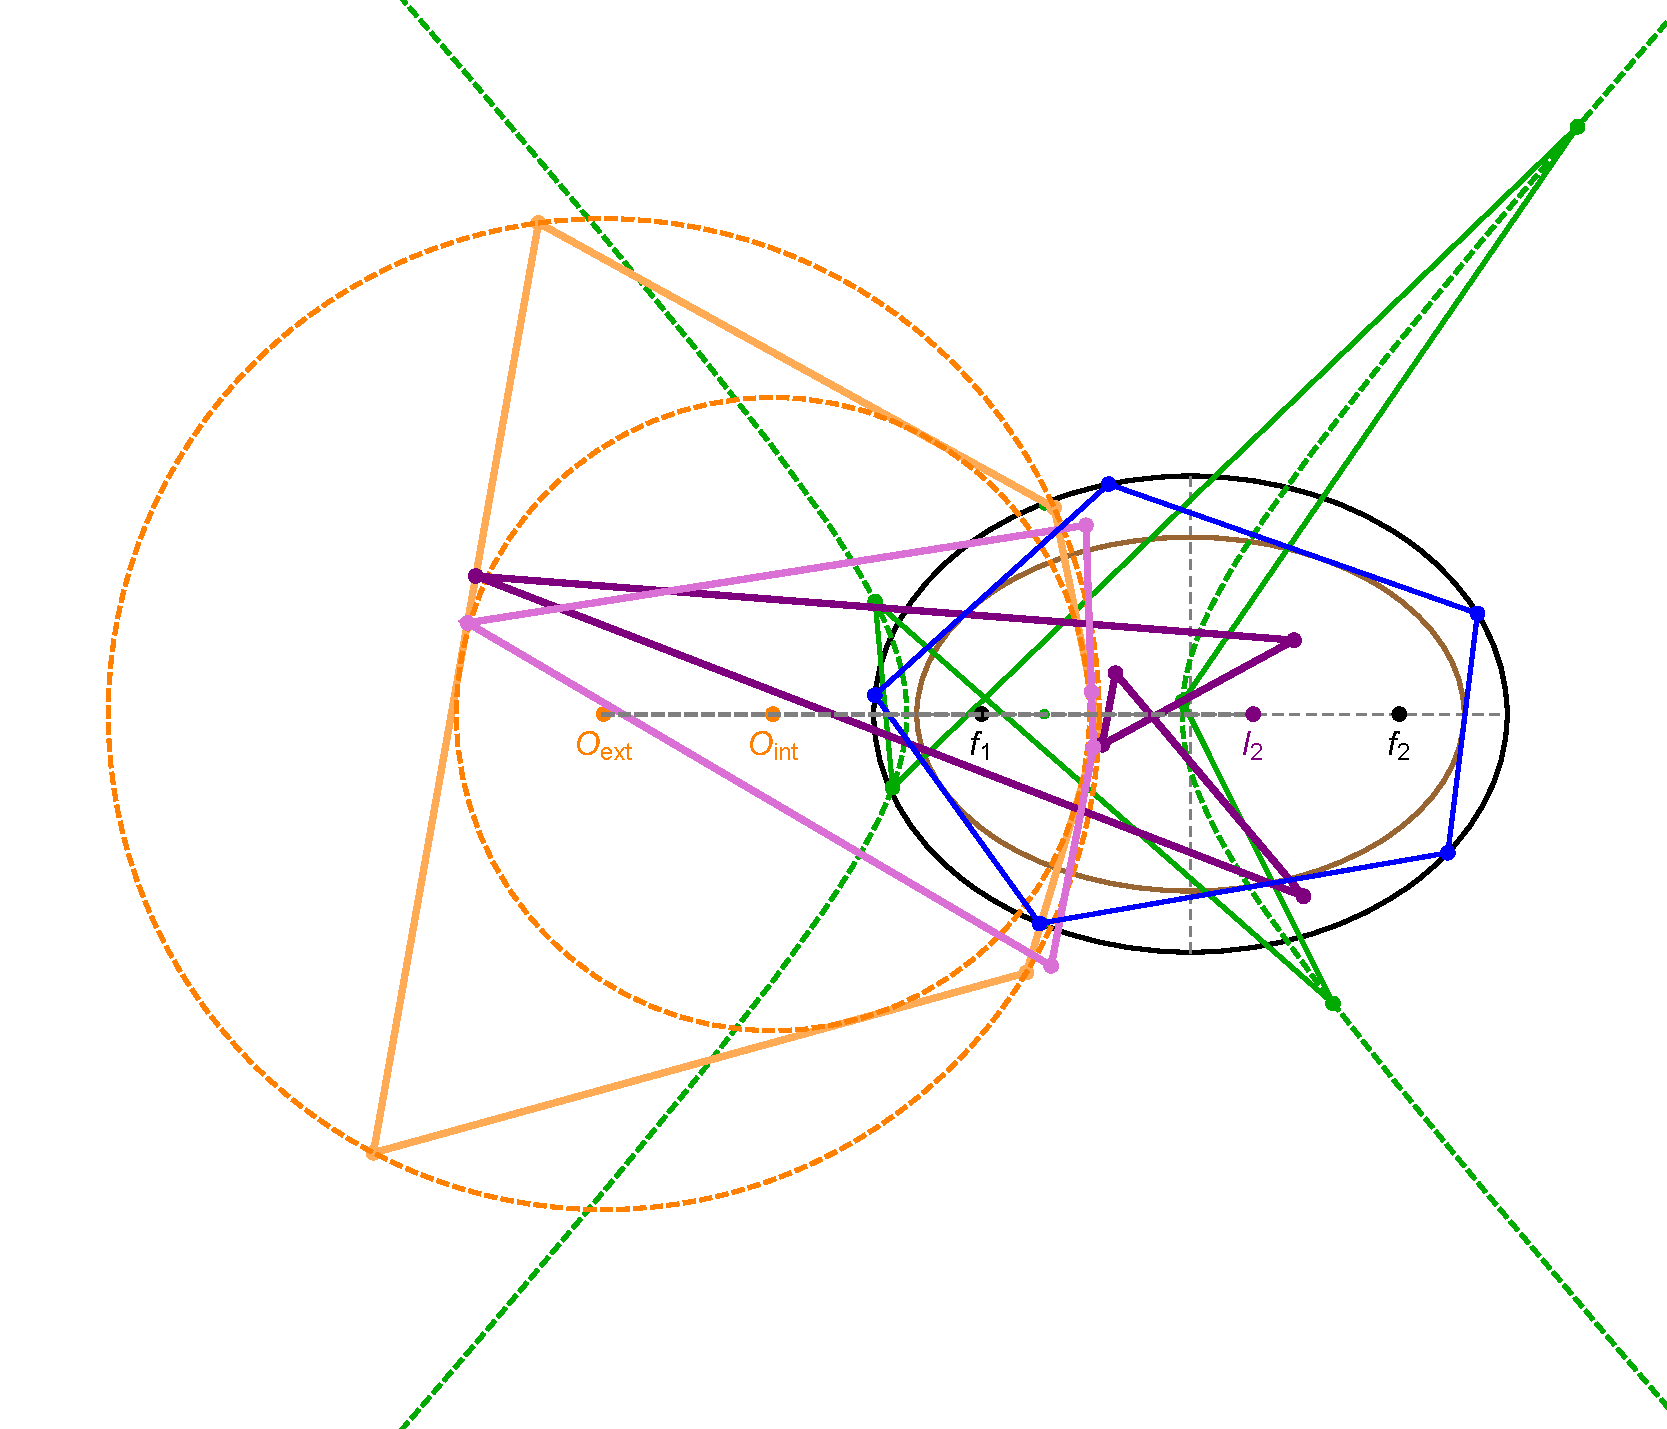
\includegraphics[width=\textwidth]{chap_05/pics/pics_05_0130_five_polys.pdf}
    \caption{The bicentric family (solid orange), its two polar images: the elliptic billiard (blue) and the hyperbolic biliard (green), and the two limiting pedal polygons (pink and purple). All but the bicentrics are equiperimetric. All conserve their sum of cosines.}
    \label{fig:five-polys}
\end{figure}


\begin{figure}
    \centering
    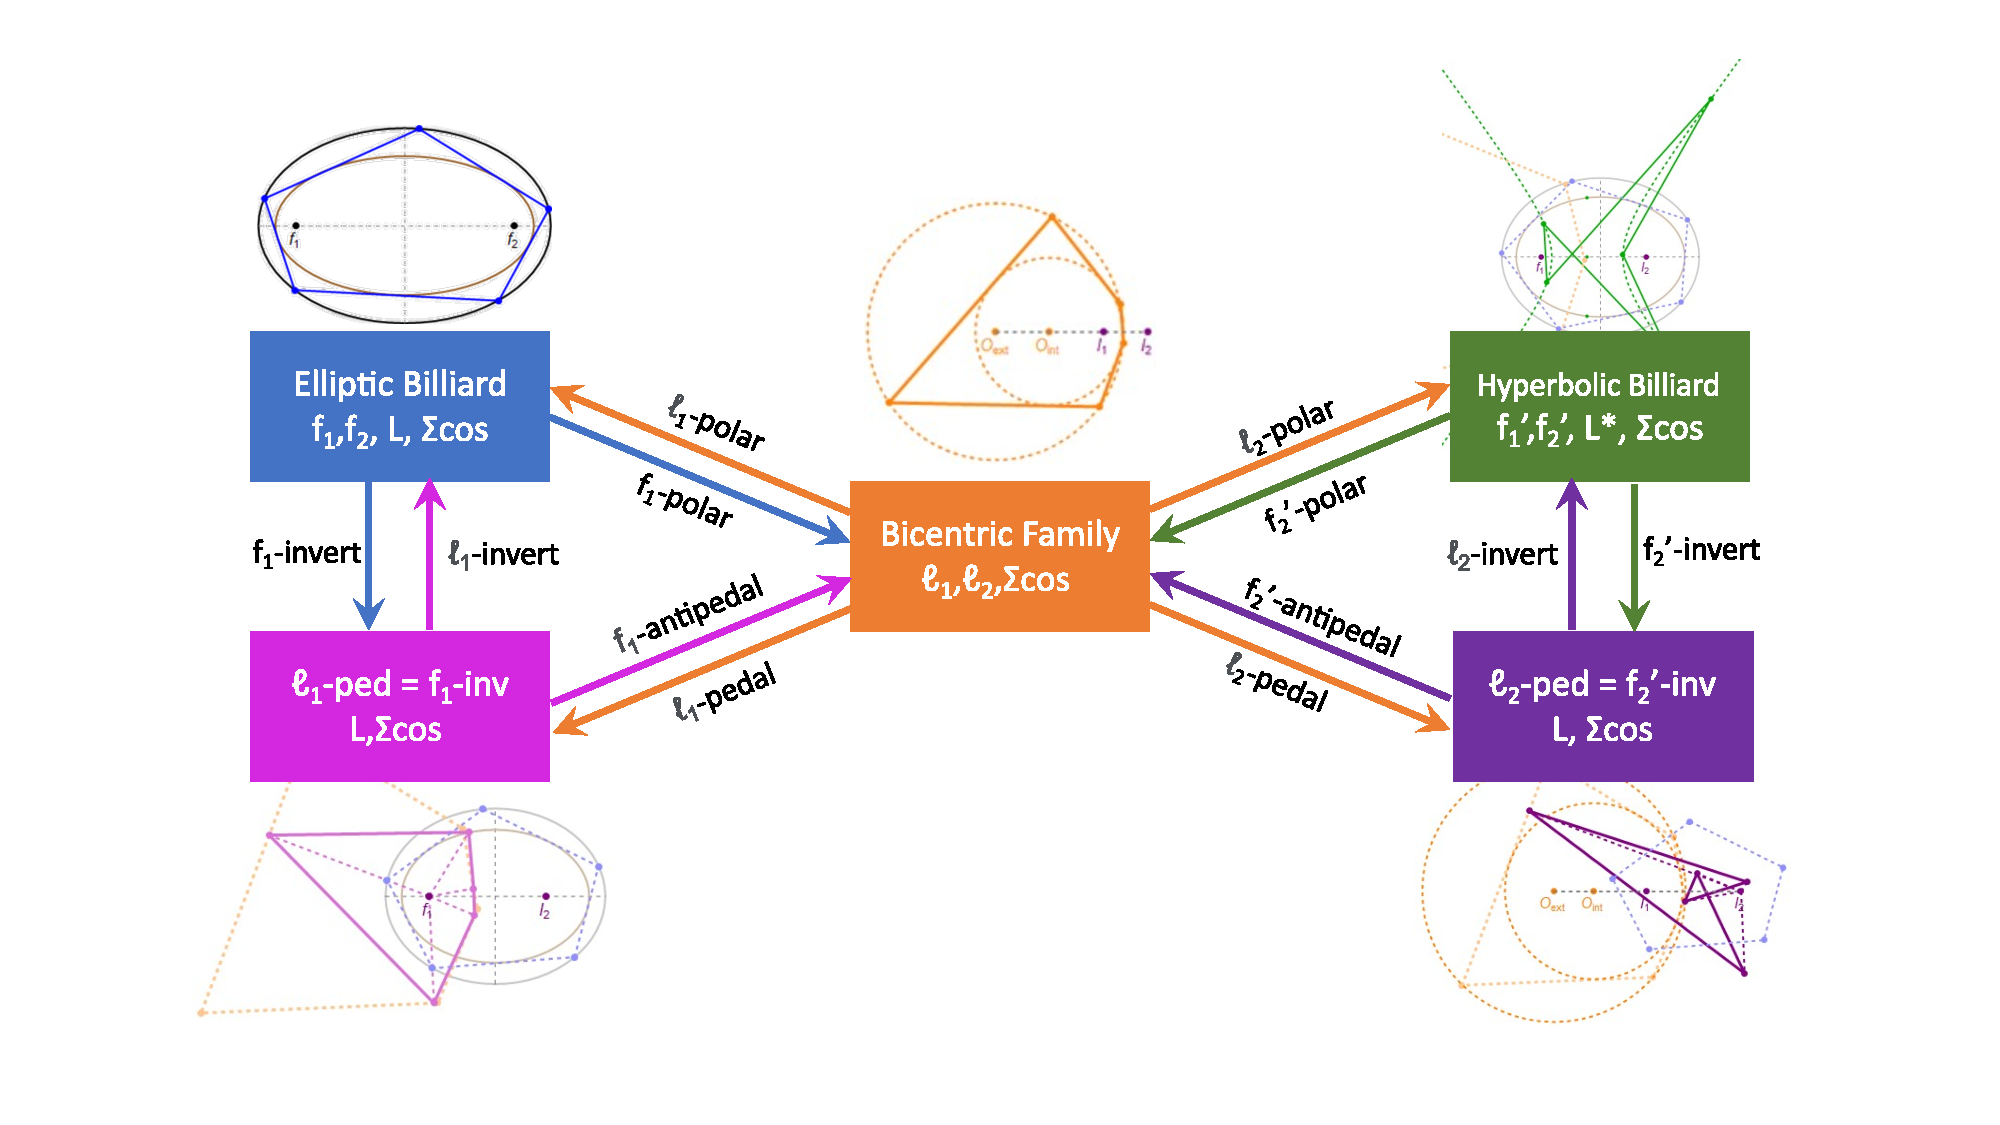
\includegraphics[trim=100 50 100 50,clip,width=\textwidth]{pics_05_0140_bicentric_diagram.pdf}
    \caption{The bicentric family (orange, center) is the hub from which four polygon families can be derived: the (i) elliptic (resp. (ii) hyperbolic) billiard with foci $f_1=\ell_1,f_2$ (resp. $f_1'$ and $f_2'=\ell_2$) is the bicentric polar image with respect to $\ell_1$ (resp. $\ell_2$); (iii) the first (resp. second) pedal is obtained with respect to $\ell_1$ (resp. $\ell_2$). These are the inversive image of the elliptic and hyperbolic billiards with respect to $l_1=f_1$ or $l_2=f_2'$, respectively. With the exception of the bicentrics, all 4 derived families conserve perimeter $L$ (in the case of the hyperbolic billiard it is the {\em signed} perimeter $L^*$ which is conserved. All 5 families conserve sum of cosines, except for $N=4$ $\ell_1$-pedals.}
    \label{fig:bicentric-diagram}
\end{figure}  

%\section{List of Videos}
%\label{sec:videos}
%\input{090_videos}

 
\section{Polar Pedal Transformations}
\label{sec:06-polar-pedal}
Consider the pair of nested circles:
 
\[\C_{int}:\;x^2+y^2=r^2,\;\;\;\C_{ext}:\;(x+d)^2+y^2=R^2\]
Their limiting points $\ell_1$ and $\ell_2$ are given by \cite[Limiting Points]{mw}:
 
 \[ \ell_1= (R^2 - d^2 - r^2 -\Delta)/(2d),\;\;\;\ell_2=(R^2 - d^2 - r^2 + \Delta)/(2 d)\]
where:
 \[ \Delta=\sqrt { \left( d+R+r \right)  \left( R-d+r \right)  \left( R+d-r
 \right)  \left( R-d-r \right) }\]

Notice $\ell_1$ (resp. $\ell_2$) is internal (resp. external) to the circle pair. Below we show that the polar image of the  $\C_{int},\C_{ext}$ pair with respect to a circle of radius $\rho$ centered on $\ell_1$ (resp. $\ell_2$) is a confocal pair of ellipses (resp. hyperbolas).

\begin{lemma}
The polar image of $\C_{int}$ with respect to $\ell_1 $ is the ellipse $\E$ centered at
 \[ \O_e=\left[  {\rho}^2\frac{d}{\Delta} +\frac{k-\Delta}{2d},0\right] \]
where $k=R^2 - d^2 - r^2$. Its semi-axes are given by:
 
\[  a^2={\rho}^4\left(\frac{2d^2r^2+ \Delta(k+\Delta)}{ 2 \Delta^2 r^2}\right),\;\;\;b^2= {\rho}^4\left(\frac{k+ \Delta}{2 \Delta r^2}\right) \]
 \end{lemma}
\noindent Note that $c^2=a^2-b^2={\rho}^4d^2/{\Delta^2}$.
 
 \begin{lemma}
 The polar image of $\C_{ext}$ with respect to $\ell_1$ is an ellipse $\E'$ confocal with $\E$ with semi-axes given by:
 
\[  a'^2= {\rho}^4\frac{(2R^2d^2 + \Delta (k'+\Delta ))}{ 2 \Delta^2 R^2},\;\;\;b'^2=  {\rho}^4\left(\frac{k'+\Delta}{ 2 \Delta R^2}\right) \]
 \end{lemma}
 \noindent where $k'=R^2 + d^2 - r^2$.
 
 \begin{lemma}
 The polar image of $\C_{int}$ with respect to $\ell_2 $ is the hyperbola $\H$ centered at
  \[  \O_h=\left[  {-\rho}^2\frac{d}{\Delta} +\frac{k+\Delta}{2d},0\right] \]
 with semiaxes given by:
 
\[  a_h^2={\rho}^4\left(\frac{  2d^2r^2-\Delta(k - \Delta)}{2  \Delta^2 r^2}\right),\;\;\;b_h^2= {\rho}^4\left(\frac{k - \Delta}{2 \Delta r^2}\right)\]
 \end{lemma}
 \noindent Note that $c_h^2=a_h^2+b_h^2={{\rho}^4d^2}/{\Delta^2}$. Note also that $c=c_h$.
 
 \begin{lemma} The polar image of $\C_{out}$ with respect to $\ell_2$ is a hyperbola $\H'$ confocal with $\H$. Its semiaxes are given by:
 
\[ a_h'^2= {\rho}^4\left(\frac{2R^2d^2 - \Delta (k' - \Delta)}{ 2 \Delta^2 R^2}\right),\;\;\; b_h'^2= {\rho}^4 \left(\frac{k' - \Delta}{ 2 \Delta R^2}\right)\]
 \end{lemma}


 
\section{Limiting Pedal Perimeters}
\label{sec:06-explicit-perimeter}
Using the identities

\begin{align*}
    sn(u+v)&={\frac {sn \left( u \right) cn \left( v \right) dn
 \left( v \right) +sn \left( v \right) cn \left( u
 \right) dn \left( u \right) }{\Delta \left( u,v \right) }}
\\
cn(u+v)&={\frac {cn \left( u \right) cn \left( v \right) -sn
 \left( u \right) sn \left( v \right) dn \left( u \right) 
dn \left( v \right) }{\Delta \left( u,v \right) }}
\\
dn(u+v)&={\frac {dn \left( u \right) dn \left( v \right) -{k}^{2}{
\it sn} \left( u \right) sn \left( v \right) cn \left( u
 \right) cn \left( v \right) }{\Delta \left( u,v \right) }}\\
\Delta(u,v)&=1-k^2 sn^2u\, sn^2v,\;\;\;  dn^2(u)+k^2sn^2(u)=1
\end{align*}
It follows that 

\[L_\pm(u)=L_\pm(0)=2 \,cn(\sigma)
sn(\sigma) \frac{\sqrt{ \delta_{\pm}R}}{k} \sum_{j=1}^{N}
  \,\frac{
  dn^2(j \sigma) }{  1-   \left(1-  dn^{2}(j \sigma) \right) 
  sn^{2}(\sigma)}
\]

\noindent where as before $\sigma=(4 \tau K)/N$.








\section{Bicentric Vertices:\torp{$N$}{N} = 3, 4}
\label{sec:06=bicentric-vertices-n34}
Consider a pair of circles
\[\mathcal{C}_1: x^2+y^2-r^2=0, \;\;\; \mathcal{C}_2: (x+d)^2+y^2-R^2=0\]

\subsection{N=3}

Let $(x_0,y_0)=(r\cos t,r\sin t) \in \mathcal{C}_1$. Let
$d^2=R(R-2r)$. Then the 3-periodic orbit is parametrized by
$\{P_1,P_2,P_3 \}, $ where
{\small  
\begin{align*}
P_1&=\left[{\frac {\cos t(2\,d R    \cos  t    +    {R}^{2}-  {d}^{2})+\Delta\,\sin t}{2\,R}}-d, {\frac {\sin t( 2d R\, \cos
 t  +  {R}^{2}-d^2) -\Delta\,\cos t }{2\,R}}\right]
\\
P_2&=\left[ {\frac { \cos t(2\,d R  \cos t     +{R}^{2}- {d}^{2})-\Delta\,\sin
 t }{2\,R}}-d,{\frac {\sin t(2d R\,  \cos
 t  +   {R}^{2}-  {d}^{2})+\Delta\,\cos t }{2\,R}}\right]
\\
 P_3&=\left[-{\frac { \left( R\cos t   -d \right)  \left( {R}^{2}-{d
}^{2} \right) }{     R^2+d^2-2\,d R\cos t }   }, {\frac 
{ -R\left(   R^2-d^2 \right) \sin t }{ R^2+d^2-2\,d R \cos
 t  }}\right]\\
 \Delta&=\sqrt { \left(  R^2+d^2-2d R\,\cos t   \right) 
 \left(   3\, R^2-d^2 +2\,d R\cos t\right) }
 \end{align*}
 }
Under the above pair of circles, the limiting points are at:

\begin{align*}
    l_1&=\left[\frac{  R^2-d^2 }{8\,d {R}^{2} }
 \left( \sqrt {   (9\,R^2-d^2)    
  (R^2-d^2)     }+3\, R^2+d^2 \right) 
,0\right]\\
l_2&=l_1-\left[\frac{\sqrt{9R^2 - d^2} (R^2-d^2)^{\frac{3}{2}}}{4R^2d}, 0\right].
\end{align*}
 
\subsection{N=4}

Let $(x_0,y_0)\in \mathcal{C}_1$. 
The Cayley condition for a pair of circles to admit Poncelet 4-periodics due to Kerawala is \cite[Poncelet's Porism, Eq. 39]{mw}:

\[ \frac{1}{(R-d)^2}+ \frac{1}{(R+d)^2}-\frac{1}{r^2}=0 \]
  
Let $P_i=[x_i,y_i]$, $i=1,...,4$ denote the vertices of a bicentric 4-periodic. Let $\alpha=R^2+d^2$ and $\beta=R^2-d^2$. The vertices are parametrized as:
 
\begin{align*}
\small
   x_{1}&=\Delta\,y_0-{\frac { \left( \beta+2\,d x_0
 \right)  \left( d \alpha  -\beta x_0 \right) }{2\,\alpha}},\\
 y_{1}&=-\Delta\,x_0+{\frac { \left( 2\,d \beta x_0+
 \alpha ^{2} \right) y_0}{2\,\alpha}}\\
x_{2}&=-\Delta\,y_0-{\frac { \left( \beta+2\,dx_0
 \right)  \left( d \beta - \beta x_0 \right) }{2\,\alpha}}\\
y_{2}&=\Delta\,x_0+{\frac {2\,d \beta y_0\,x_0+
 \alpha ^{2}y_0}{2\,\alpha}}\\
%
 x_3&= \frac{  ((( x_0^2 \alpha \beta - 4  x_0^2 \alpha^2 + 3/2 \beta^3 - 2 \beta^2 \alpha) \sqrt{2 \alpha - 2 \beta} + \beta (2 \Delta \alpha  y_0 + 8 \alpha^2  x_0 - 8 \alpha \beta  x_0 + \beta^2  x_0)) \beta)}{(4 (\sqrt{2 \alpha - 2 \beta} \alpha  x_0 + \beta (\beta - 2 \alpha)/2)^2)}\\
 y_3&=\frac{\alpha \beta (\alpha (2  x_0  y_0 \alpha + \beta ( x_0  y_0 - 2 \Delta)) \sqrt{2 \alpha - 2 \beta} + (4 \Delta  x_0 - 2 \beta  y_0) \alpha^2 - 2 \Delta \alpha \beta  x_0 + \beta^3  y_0)}{(2 \sqrt{2 \alpha - 2 \beta} \alpha  x_0 - 2 \alpha \beta + \beta^2)^2}\\
 x_4&=-\frac{((( x_0^2 \alpha \beta - 4  x_0^2 \alpha^2 + 3/2 \beta^3 - 2 \beta^2 \alpha) \sqrt{2 \alpha - 2 \beta} + \beta (-2 \Delta \alpha  y_0 + 8 \alpha^2  x_0 - 8 \alpha \beta  x_0 + \beta^2  x_0)) \beta)}{(4 (\sqrt{2 \alpha - 2 \beta} \alpha  x_0 + \beta (\beta - 2 \alpha)/2)^2)}\\
 y_4&=\frac{(\alpha (2  x_0  y_0 \alpha + \beta ( x_0  y_0 + 2 \Delta)) \sqrt{2 \alpha - 2 \beta} + (-4 \Delta  x_0 - 2 \beta  y_0) \alpha^2 + 2 \Delta \alpha \beta  x_0 + \beta^3  y_0) \beta}{(2 \sqrt{2 \alpha - 2 \beta} \alpha  x_0 - 2 \alpha \beta + \beta^2)^2}\\
 \Delta&=\frac{\sqrt{-2\sqrt{2\alpha - 2\beta}\; \alpha x_0\beta^2 - 2 x_0^2\alpha^3 + 2 x_0^2\alpha^2\beta + \alpha^2\beta^2 + \alpha\beta^3 - \beta^4}}{ (2\alpha}
\end{align*}

Under the above pair of circles, the limiting points are at:
\begin{align*}
    l_1=\left[\frac{R^2 - d^2}{2d}, 0\right],\;\;\; l_2=  \left[\frac{d(R^2-d^2)}{R^2 + d^2}, 0\right]
\end{align*} 

\section{Limiting Pedal Perimeters for \torp{$N$}{N} =3 and \torp{$N$}{N} =4}
\label{sec:06-pedal-perimeters-n34}
 Below we consider 3- and 4-periodics in the confocal pair where $a,b$ are the semi-axes of the outer ellipse has axes $(a,b)$. Below, set $\delta=\sqrt{a^4-a^2 b^2+b^4}$ and $c^2=a^2-b^2$.

\subsection{N=3 case}

\begin{figure}
    \centering
    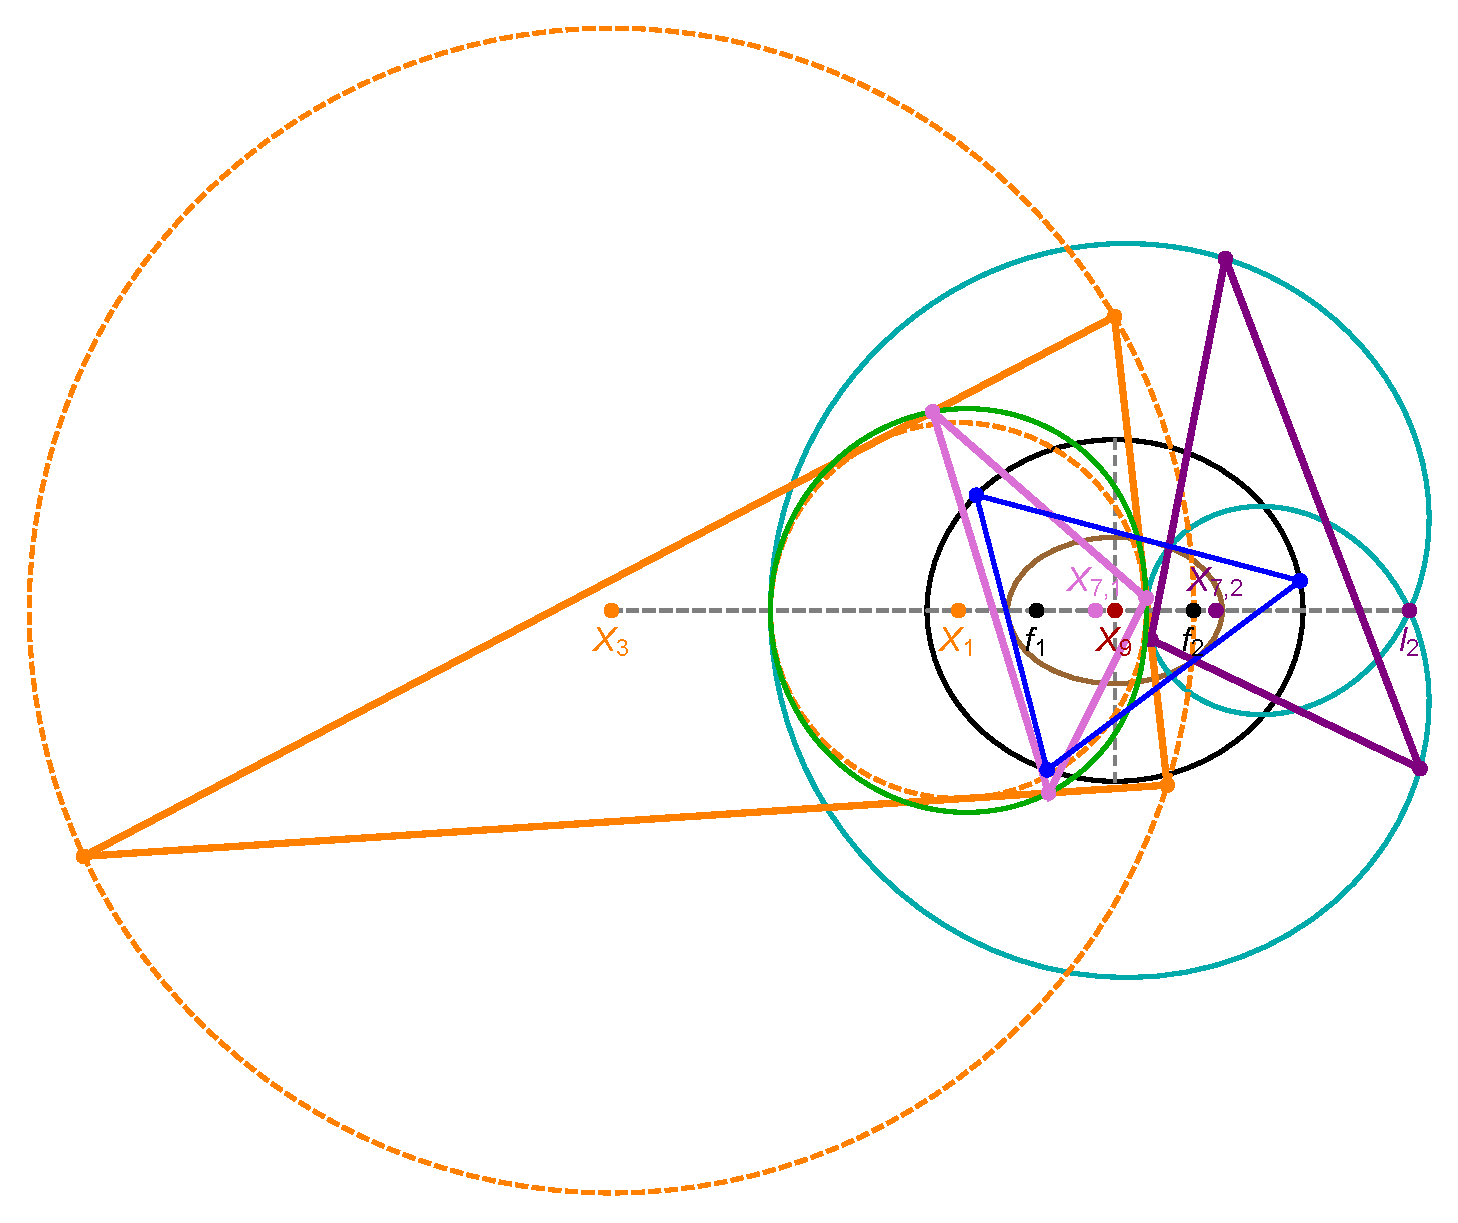
\includegraphics[width=.9\textwidth]{pics_05_0060_n3.pdf}
    \caption{N=3 case: the bicentric family (solid orange) is the poristic family \cite{gallatly1914-geometry}. Its sum of cosines is invariant and equal to those of the two limit point pedals (pink and purple). The Gergonne points $X_{7,1}$ and $X_{7,2}$ of each pedal are stationary. \href{https://bit.ly/379HU8l}{live}}
    \label{fig:n3}
\end{figure}

Referring to Figure~\ref{fig:n3}, the perimeter $L^\dagger$ of the inversive polygon for the $N=3$ family, originally derived in  \cite[Prop. 4]{reznik2020-n3-focus-inversive} is given by:


\[L^\dagger=L_+=\rho^2 \frac {\sqrt { \left( 8\,{a}^{4}+4\,{a}^{2}{b}^{2}+2\,{b}^{4}
 \right) \delta+8\,{a}^{6}+3\,{a}^{2}{b}^{4}+2\,{b}^{6}}}{{a}^{2}{b}^{
2}}\]

By Corollary~\ref{cor:inv-per}, this is equal to the perimeter $L_-$ of the bicentric pedal with respect to the focal limiting point.

\begin{align*}
    L_{-} &= {\frac {  \left( 9\,{R}^{2}-{d}^{2} \right)  \left( {R}^{2}-{d}^{2}
 \right) \sqrt {2}\rho^2}{16\,{R}^{4}d}\sqrt {- \left( {R}^{2}-{d}^{2}
 \right) ^{{\frac{3}{2}}}\sqrt {9\,{R}^{2}-{d}^{2}}+ 3R^4 + 6R^2d^2 - d^4}}\\
R&=(2a^4 - 2a^2b^2 + b^4 + (2a^2 -b^2)\delta  )a\rho^2/b^6,\;\;
d=(2a^2 - b^2 + 2\delta)c\rho^2a^2/b^6
\end{align*}

The perimeter $L_+$ of the bicentric pair with respect to the non-focal limiting point is given by:

\begin{align*}
    L_{+} &= {\frac { \left( 9\,{R}^{2}-{d}^{2} \right)  \left( {R}^{2}-{d}^{2}
 \right) \sqrt {2}\rho^2}{16\,{R}^{4}d}\sqrt { \left( {R}^{2}-{d}^{2}
 \right) ^{{\frac{3}{2}}}\sqrt {9\,{R}^{2}-{d}^{2}}+ 3R^4 + 6R^2d^2 - d^4}}\\
R&=(2a^4 - 2a^2b^2 + b^4 + (2a^2 -b^2)\delta  )a\rho^2/b^6,\;\;
d=(2a^2 - b^2 + 2\delta)c\rho^2a^2/b^6
\end{align*}

The sum of cosines of a triangle is given by $1+r/R$ and is therefore constant for the $N=3$ bicentric family. Let $\theta'_i$ denote the angles of the bicentric polygon. The sum  its cosines can be derived as:

\begin{equation}
\sum\cos\theta' = 1+\frac{r}{R} = \frac{3R^2 - d^2}{2R^2}
\label{eq:bic-cos}
\end{equation}

\begin{proposition}
The sum of cosines for the first and second $N=3$ bicentric pedals are constant and identical to \eqref{eq:bic-cos}.
\end{proposition}

Note: in terms of the associated elliptic billiard parameters, this is given by \cite[Prop. 6]{reznik2020-n3-focus-inversive}:

\[\sum\cos{\theta^\dagger}_{(N=3)}=\frac{\delta (a^2+c^2-\delta)}{a^2c^2} \]


\begin{proof} Using CAS, it follows from  straightforward calculations with the orbit parametrized in Appendix \ref{app:bicentric-vertices-n34}.
\end{proof}

The two limiting pedals have stationary Gergonne points $X_7$. The first one was derived in \cite[Proposition 1]{garcia2020-self-intersected}:

\[ X_{7,1}=\left[c\left(1-\frac{\rho^2}{\delta+c^2}\right),0\right]  \]


\[X_{7,1} =\frac{ (R^2 - d^2)((R^2 - d^2)^{3/2}\sqrt{9R^2 - d^2} + 3R^4 + 6R^2d^2 - d^4)}{16R^4d}\]

%\[X_{7,2}=-\frac{(R^2  -d^2) ((R^2 - %d^2)^{3/2}\sqrt{9R^2 - d^2} - 3R^4 - 6R^2d^2 + d^4)}{16d R^4}
%\]
\subsection{N=4 case}

\begin{figure}
    \centering
    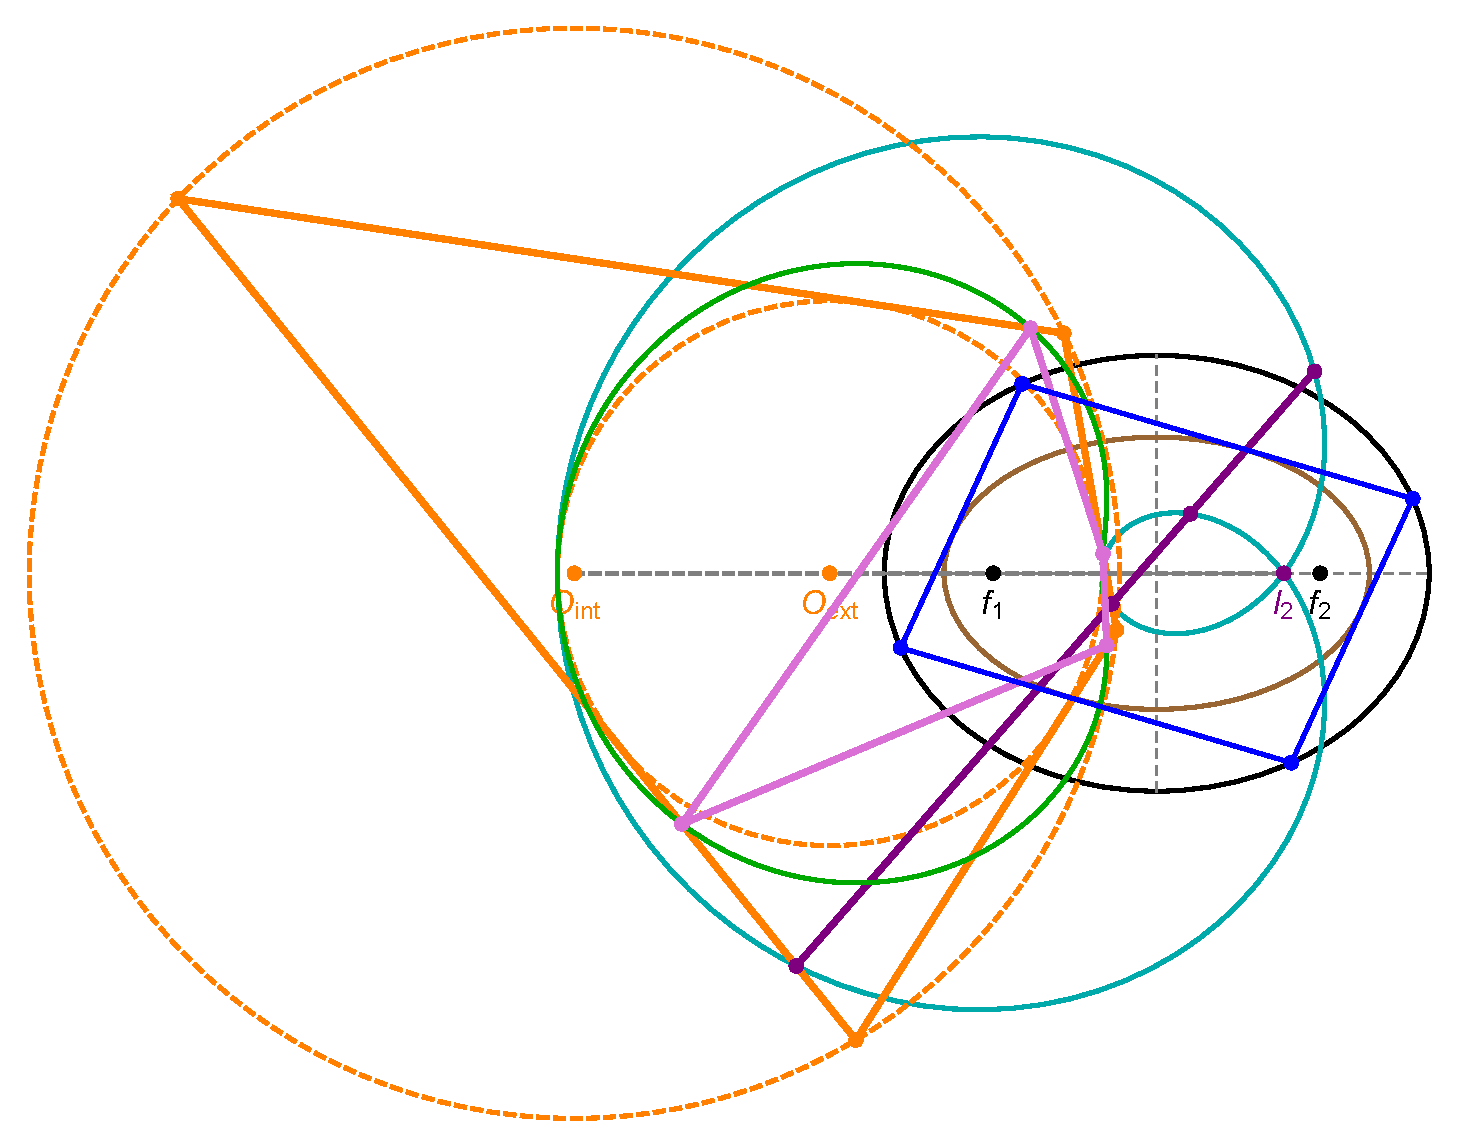
\includegraphics[width=.9\textwidth]{pics_05_0050_n4.pdf}
    \caption{In the N=4 case, remarkable things happen: (i) the sum of cosines of the $f_1$-pedal (pink) is not constant; (iii) its perimeter is the same as the corresponding billiard 4-periodic; (iv) the vertices of the $l_2$-pedal (purple) are collinear and (v) the sum of its cosines is 4. \href{https://youtu.be/fZe6elRTfeA}{Video}}
    \label{fig:n4}
\end{figure}

Referring to Figure~\ref{fig:n4}, the perimeter $L^\dagger$ of the inversive polygon for billiard 4-periodics was originally derived in  \cite[Prop. 18]{garcia2020-self-intersected}. It is identical to the perimeter of 4-periodics themselves and given by:

\begin{equation}
    L^\dagger= L_{+,N=4}= \,{\frac {4\sqrt {{a}^{2}+{b}^{2}}}{{b}^{2}}}
\label{eqn:inv-per-n4} 
\end{equation}

\begin{proposition}\label{prop:bicentricpedalN4}
In the $N=4$ family, the vertices of the bicentric pedal with respect to the non-focal limiting point are collinear.
\end{proposition}

\begin{proof}
The polar image of the bicentric family with respect to $\ell_2$ is a pair of confocal hyperbolas, see \cref{app:bicentric-to-confocal}, i.e., the polar image of bicentric 4-periodics is a billiard family. It can be shown its vertices are concyclic with the two hyperbolic foci $f_1',f_2'$, one of which coincides with $\ell_2$. Therefore, the inversion of said vertices with respect to $\ell_2$ is a set of collinear points.
\end{proof}

As before, Equation~\ref{eqn:inv-per-n4} is the same as the perimeter of the first bicentric pedal. The perimeter $L_+$ of the non-focal bicentric pedal is given by:

\[ L_{-,N=4} = \frac{4a^2}{b^2 c} \]

Regarding the sum of cosines, it is well-known a circle-inscribed quadrilateral has supplementary opposing angles, i.e.:

\begin{observation}
The sum of cosines of a bicentric N=4 family is null.
\end{observation}

Since the second bicentric pedal is a degenerate polygon:

\begin{observation}
The sum of cosines of the second limiting pedal to the N=4 bicentric family is equal to 4.
\end{observation}

 

\section{Exercises}
\label{sec:06-exercises}


\begin{exercise}\label{exer:51}
A ``focus-inversive'' polygon, is a $N$-gon whose vertices are inversions of elliptic billiard N-periodic vertices with respect to a circle of radius $\rho$ centered on one focus. See \cref{fig:chap5_inversiveN3}.

\begin{figure}[H]
    \centering
    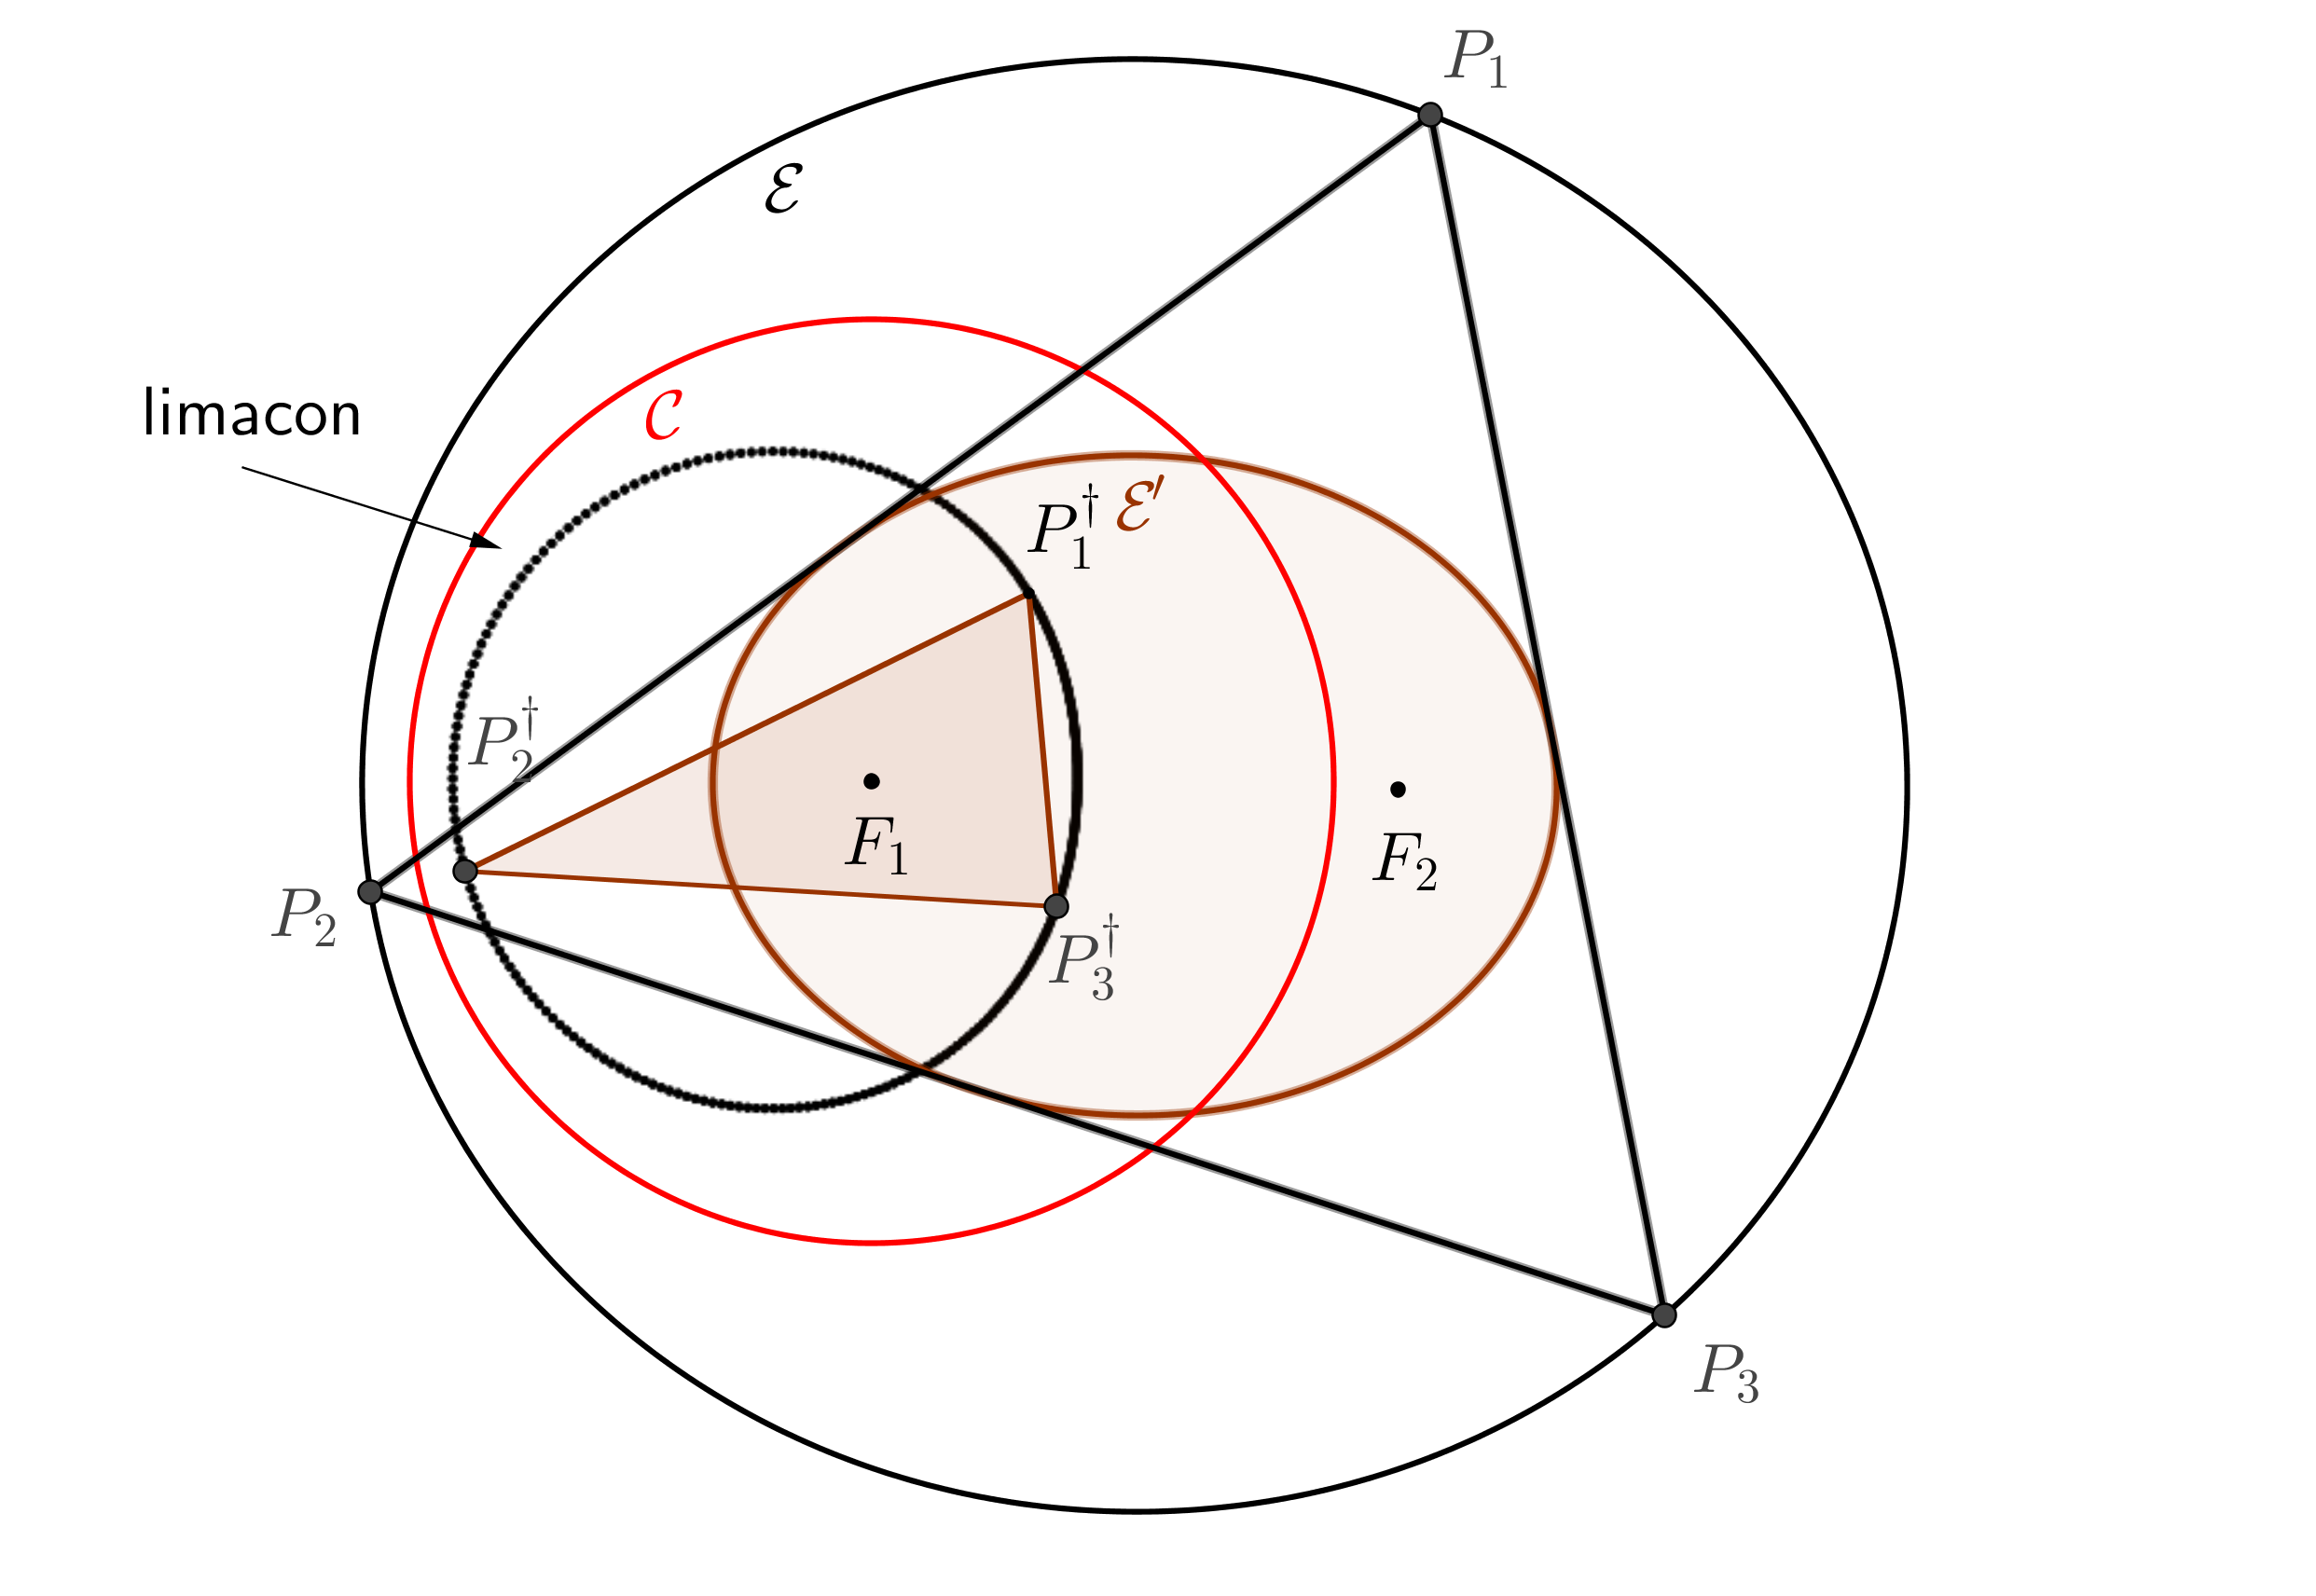
\includegraphics[scale=0.5]{pics_05_0910_inversivoN3.png}
    \caption{Inversive triangle $P_1^{\dag}P_2^{\dag}P_3^{\dag}$ of 3-billiard orbit $P_1P_2P_3$.}
    \label{fig:chap5_inversiveN3}
\end{figure}

It is well known the inversion of an ellipse with respect to a focus-centered unit circle is Pascal's Limaçon $\mathcal{L}(t)$ \cite{ferreol2020-limacon}, given by:

\[ \mathcal{L}(t)=\left[-a \cos{t} (\varepsilon  \cos{t}+1)-c,a \sin{t} (\varepsilon \cos{t}+1)\right],\;\;0{\leq}t{\leq}2\pi
\]

\noindent Therefore:

For any $N$, the focus-inversive family is inscribed in $\mathcal{L}(t)$.

\noindent i) Show that 
the perimeter $L^\dagger$ of the N=3 focus-inversive family is invariant and given by:

\[L^\dagger=\rho^2 \frac {\sqrt { \left( 8\,{a}^{4}+4\,{a}^{2}{b}^{2}+2\,{b}^{4}
 \right) \delta+8\,{a}^{6}+3\,{a}^{2}{b}^{4}+2\,{b}^{6}}}{{a}^{2}{b}^{
2}}\]
 
\noindent ii) Show that for $N=3$, the sum of focus-inverse spoke lengths $\sum{1/d_{1,i}}$ is invariant and given by:

\[  \sum{1/d_{1,i}}=\frac {{a}^{2}+{b}^{2}+\delta}{a{b}^{
2}}
\] 

\noindent iii) Show that for $N=3$, the sum of focus-inversive cosines $\sum\cos{\theta_{1,i}^\dagger}$ is given by:
\[\sum\cos{\theta_{1,i}^\dagger}=\frac{\delta (a^2+c^2-\delta)}{a^2c^2}\]

%\noindent iv) Show that the product of the areas for $N=3$ of the inversive triangle is invariant under the family of 3-periodic orbits.

\end{exercise}


\begin{exercise}\label{exer:52} Let $X_1^{\dag}$ be the incenter of the inversive triangle $P_1^{\dag}P_2^{\dag}P_3^{\dag}$. 

Show that the locus of $X_1^\dag$ is the circle given by:
\begin{align*}
C_1^\dagger=&\left[c\left(-1+\rho^2\frac{-2a^2+b^2+2\delta}{2b^4}\right), 0\right]\\
R_1^\dagger=&\rho^2\frac{b^4 -2\delta^2+(2a^2-b^2)\delta}{2ab^4}
\end{align*}
\end{exercise}



\begin{exercise}\label{exer:53} Referring to \cref{fig:chap5_inversiveN3} consider the envelope $\mathcal{L}^\dag$ of the family of lines
$\ell_{12}=P_1^\dag P_2^\dag$.

Show that when the limaçon $\mathcal{L}$ is a convex curve, the envelope $\mathcal{L}^\dag$ is a regular convex curve.

Conclude that  $\{ \mathcal{L}, \mathcal{L}^\dag\}$ is Poncelet pair having  the triangles orbits $P_1^{\dag}P_2^{\dag}P_3^{\dag}$ as 3-periodics.
 
 
\end{exercise}
